%%%% ijcai25.tex

\typeout{IJCAI--25 Instructions for Authors}

% These are the instructions for authors for IJCAI-25.

\documentclass{article}
\pdfpagewidth=8.5in
\pdfpageheight=11in

% The file ijcai25.sty is a copy from ijcai22.sty
% The file ijcai22.sty is NOT the same as previous years'
\usepackage{ijcai25}

% Use the postscript times font!
\usepackage{times}
\usepackage{soul}
\usepackage{url}
\usepackage[hidelinks]{hyperref}
\usepackage[utf8]{inputenc}
\usepackage[small]{caption}
\usepackage{graphicx}
\usepackage{amsmath}
\usepackage{amsthm}
\usepackage{booktabs}
\usepackage{algorithm}
\usepackage{algorithmic}
\usepackage[switch]{lineno}

% Comment out this line in the camera-ready submission
% \linenumbers

\urlstyle{same}

% the following package is optional:
%\usepackage{latexsym}

% See https://www.overleaf.com/learn/latex/theorems_and_proofs
% for a nice explanation of how to define new theorems, but keep
% in mind that the amsthm package is already included in this
% template and that you must *not* alter the styling.
\newtheorem{example}{Example}
\newtheorem{theorem}{Theorem}
\newtheorem{lemma}{Lemma}
\newtheorem{corollary}{Corollary}
\newtheorem{observation}{Observation}
\newtheorem{assumption}{Assumption}


% % OUR STUFF
% % nicer fonts
% % \usepackage[bitstream-charter]{mathdesign}

% % \usepackage[sfdefault,lf]{carlito}
% % \usepackage[T1]{fontenc}
% % \renewcommand*\oldstylenums[1]{\carlitoOsF #1}

% \usepackage[sfdefault,scaled=.85]{FiraSans}
% \usepackage[T1]{fontenc}
% \usepackage{textcomp}
% \usepackage[cmintegrals]{newtxsf}

% % seb's name
\usepackage[utf8]{inputenc}

% % for coloured text
\usepackage{xcolor}
% % for nicer tables
\usepackage{booktabs}
% % for newtheorem
% \usepackage{amsthm}
% % for code
\usepackage{listings}
% % better tt font
\usepackage{inconsolata}
% % for plots
\usepackage{tikz}
% % also for plots
\usepackage{pgfplots}
% % for text in mathmode
\usepackage{amsmath}
% % nicer fonts
\usepackage{microtype}
% % for including algorithms
\usepackage{algorithm}
% % for strikeout
\usepackage{amssymb}
\usepackage[titletoc]{appendix}
 \usepackage{cancel}
 \usepackage{multirow}
\usepackage{subfig}
% \usepackage{natbib}

\usepackage{pgfplots}
\usepgfplotslibrary{colorbrewer}
\pgfplotsset{compat = 1.15, cycle list/Set1-8} 
\usetikzlibrary{pgfplots.statistics, pgfplots.colorbrewer} 
\usepackage{pgfplotstable}

% % \usepackage{subcaption}
% % \usepackage{tikz}
% % \definecolor{pixel 0}{HTML}{FFFFFF}
% % \definecolor{pixel 1}{HTML}{FF0000} % red




\newcommand{\citeA}[1]{\citeauthor{#1} [\citeyear{#1}]} 
\newcommand{\ac}[1]{\textcolor{red}{AC: #1}}
\newcommand{\dc}[1]{\textcolor{magenta}{DC: #1}}

\newcommand{\ch}[1]{\textcolor{blue}{CH: #1}}
% \newcommand{\jk}[1]{\textcolor{blue}{JK: #1}}
% \newcommand{\tw}[1]{\texttt{#1}}
% \newcommand{\dcc}{\textsc{DCC}}
\newcommand{\name}{\textsc{Reducer}}
\newcommand{\magicpopper}{\textsc{MagicPopper}}
\newcommand{\popper}{\textsc{Popper}}
\newcommand{\popperplus}{\textsc{Popper+}}
\newcommand{\combo}{\textsc{Combo}}
\newcommand{\dcc}{\textsc{DCC}}
\newcommand{\metagol}{\textsc{Metagol}}
\newcommand{\ilasp}{\textsc{ILASP}}
\newcommand{\ale}{\textsc{Aleph}}
\newcommand{\progol}{\textsc{Progol}}
\newcommand{\aspal}{\textsc{Aspal}}
\newcommand{\foil}{\textsc{Foil}}
\newcommand{\aspsynth}{\textsc{ASPSynth}}
% \newcommand{\dac}{D\&C}
% \newcommand{\sac}{S\&C}

% \lstset{
%     % cool font
%     basicstyle=\ttfamily\small,
%     % makes it look better
%     columns=flexible
% }

\theoremstyle{definition}
\newtheorem{definition}{Definition}
\newtheorem{myexample}{Example}
% % \newtheorem{theorem}{Theorem}
\newtheorem{proposition}{Proposition}

% \newenvironment{code}
% {
% \ttfamily
% \begin{center}
% \begin{tabular}{l}
% }
% {
% \end{tabular}
% \end{center}
% \par
% }


% make an algorithm look ok
\lstnewenvironment{myalgorithm}[1][] %defines the algorithm listing environment
{
    \lstset{ %this is the stype
        basicstyle=\normalfont\ttfamily,
        showspaces=false,               % show spaces adding particular underscores
        showstringspaces=false,         % underline spaces within strings
        mathescape=true,
        numbers=left,
        escapeinside={*}{*},
        columns=flexible,
        numbersep=2pt,        % default 10pt
        keywordstyle=\bfseries,
        keywords={,and, return, not, def, in, if, elif, else, for, foreach, while, continue,break,}
        numbers=left,
        xleftmargin=.0\textwidth,
        #1 % this is to add specific settings to an usage of this environment (for instnce, the caption and referable label)
    }
}
{}

\usepackage{pgfkeys}
    \newenvironment{customlegend}[1][]{%
        \begingroup
        \csname pgfplots@init@cleared@structures\endcsname
        \pgfplotsset{#1}%
    }{%
        \csname pgfplots@createlegend\endcsname
        \endgroup
    }%
    \def\addlegendimage{\scriptsize\csname pgfplots@addlegendimage\endcsname}
\usepackage{comment}

% Following comment is from ijcai97-submit.tex:
% The preparation of these files was supported by Schlumberger Palo Alto
% Research, AT\&T Bell Laboratories, and Morgan Kaufmann Publishers.
% Shirley Jowell, of Morgan Kaufmann Publishers, and Peter F.
% Patel-Schneider, of AT\&T Bell Laboratories collaborated on their
% preparation.

% These instructions can be modified and used in other conferences as long
% as credit to the authors and supporting agencies is retained, this notice
% is not changed, and further modification or reuse is not restricted.
% Neither Shirley Jowell nor Peter F. Patel-Schneider can be listed as
% contacts for providing assistance without their prior permission.

% To use for other conferences, change references to files and the
% conference appropriate and use other authors, contacts, publishers, and
% organizations.
% Also change the deadline and address for returning papers and the length and
% page charge instructions.
% Put where the files are available in the appropriate places.


% PDF Info Is REQUIRED.

% Please leave this \pdfinfo block untouched both for the submission and
% Camera Ready Copy. Do not include Title and Author information in the pdfinfo section
\pdfinfo{
/TemplateVersion (IJCAI.2025.0)
}

\title{Efficient Rule Induction by Ignoring Pointless Rules}


% % Single author syntax
% \author{
%     Author Name
%     \affiliations
%     Affiliation
%     \emails
%     email@example.com
% }

% Multiple author syntax (remove the single-author syntax above and the \iffalse ... \fi here)
% \iffalse
\author{
Andrew Cropper$^1$
\and
David M. Cerna$^2$
\affiliations
$^1$University of Oxford\\
$^2$Czech Academy of Sciences Institute of Computer Science (CAS ICS), Prague, Czechia
\emails
andrew.cropper@cs.ox.ac.uk,
dcerna@cs.cas.cz
}

\begin{document}

\maketitle


\begin{abstract}
The goal of inductive logic programming (ILP) is to find a set of logical rules that generalises training examples and background knowledge.
We introduce an ILP approach that identifies \emph{pointless} rules.
A rule is pointless if it contains a redundant literal or cannot discriminate against negative examples. 
We show that ignoring pointless rules allows an ILP system to soundly prune the hypothesis space.
Our experiments on multiple domains, including visual reasoning and game playing, show that our approach can reduce learning times by 99\% whilst maintaining predictive accuracies.
\end{abstract}

\section{Introduction}

The goal of inductive logic programming (ILP) is to induce a hypothesis (a set of logical rules) that generalises training examples and background knowledge (BK) \cite{mugg:ilp,ilpintro}.

To illustrate ILP, suppose we have BK with the relations \emph{succ/2}, \emph{lt/2}, \emph{gt/1}, \emph{int/1}, \emph{even/1}, \emph{odd/1} and the following positive ($E^+$) and negative ($E^-$) examples:

\begin{center}
\begin{tabular}{l}
\emph{E$^+$ = \{f(5), f(7)\}}\\
\emph{E$^-$ = \{f(2), f(3), f(4), f(6), f(8), f(9)\}}\\
\end{tabular}
\end{center}

\noindent
Given these inputs, we might want to learn a rule such as:
\begin{center}
\begin{tabular}{l}
        \emph{$r_1$ = f(A) $\leftarrow$ odd(A), gt(A,3), lt(A,8)}  
\end{tabular}
\end{center}
\noindent
This rule says that \emph{f(A)} is true if $A$ is odd, greater than 3, and less than 8.

A learner searches by testing rules on the examples and using the outcome to guide the search.
For instance, suppose a learner tests the rule:
\begin{center}
\begin{tabular}{l}
        \emph{f(A) $\leftarrow$ even(A)}    
\end{tabular}
\end{center}
\noindent
This rule is too specific because it does not entail any positive example. 
Therefore, a learner can ignore its specialisations, such as:
\begin{center}
\begin{tabular}{l}
        \emph{f(A) $\leftarrow$ even(A), gt(A,2)}    
\end{tabular}
\end{center}
\noindent
Similarly, suppose a learner tests the rule:
\begin{center}
\begin{tabular}{l}
        \emph{$r_2$ = f(A) $\leftarrow$ odd(A), int(A)}
\end{tabular}
\end{center}
\noindent
This rule is too general because it entails two negative examples (\emph{f(3)} and \emph{f(9)}).
Therefore, a learner can ignore its generalisations.
A learner will not necessarily ignore its specialisations because one could still be helpful, such as:
\begin{center}
\begin{tabular}{l}
        \emph{$r_3$ = f(A) $\leftarrow$ odd(A), int(A), gt(A,3), lt(A,8)}
\end{tabular}
\end{center}
\noindent
This rule entails all the positive and none of the negative examples.

Although seemingly useful, we argue that $r_2$ and $r_3$ are pointless because \emph{odd(A)} implies \emph{int(A)}, so we can remove \emph{int(A)} whilst preserving semantics.
We call such rules \emph{reducible} rules.

Now consider the rule:
\begin{center}
\begin{tabular}{l}
        \emph{f(A) $\leftarrow$ lt(A,B)}    
\end{tabular}
\end{center}
\noindent
This rule entails all the positive and all the negative examples. 
Therefore, a learner can ignore its generalisations.
However, although it entails all the negative examples, we cannot ignore its specialisations as one might still be a good rule, such as $r_1$.

Now consider the specialisation:
\begin{center}
\begin{tabular}{l}
        \emph{f(A) $\leftarrow$ lt(A,10)}    
\end{tabular}
\end{center}
\noindent
This rule entails all the positive and negative examples, so a learner can ignore its generalisations.
However, unlike the previous rule, a learner can ignore its specialisations.
The reason is that the literal \emph{lt(A,10)} implies all the negative examples, i.e. there is no negative example greater than 10.
Moreover, this literal cannot be further specialised (except grounding the variable $A$ and thus being pointless). 
We call such rules \emph{indiscriminate} rules. 

In this paper, we show that ignoring pointless (reducible and indiscriminate) rules allows us to efficiently and soundly prune the hypothesis space and thus improve learning performance.
Although existing approaches find reasons why a rule fails on examples, such as having erroneous literals \cite{mugg:metagold,musper} or rules  \cite{mis,prosynth}, they do not find reducible or indiscriminate rules.
We expand on the novelty in Section \ref{sec:related}.

To explore our idea, we use the \emph{learning from failures} (LFF) setting \cite{popper}.
LFF frames the ILP problem as an Answer Set Programming problem (ASP) \cite{asp}, where each (stable) model to the ASP problem represents a hypothesis.
The goal of an LFF learner is to accumulate constraints to restrict the hypothesis space.
We build on the LFF system \popper{} \cite{popper,maxsynth}, which can learn optimal and recursive hypotheses from noisy data. 
We enable \popper{} to identify pointless rules and build constraints from them to guide subsequent searches.
We call our system \name{}.

\subsubsection*{Novelty and Contributions}
The novelty of this paper is \emph{identifying pointless rules and building constraints from them to prune the hypothesis space of an ILP system}.
The impact, which we demonstrate on multiple domains, is vastly reduced learning times.
% Moreover, as the idea connects many areas of AI, including machine learning, logic programming, and constraint satisfaction, we hope the idea interests a broad audience.
Overall, we contribute the following:

\begin{itemize}
\item We define two types of pointless rules: \emph{reducible} and \emph{indiscriminate}.
We show that specialisations of reducible rule are also reducible (Proposition \ref{prop:redu_specs}).
Likewise, we show that specialisations of indiscriminate rules are also indiscriminate (Proposition \ref{prop:indi_specs}).
Finally, we show that a hypothesis with a reducible or indiscriminate rule is not optimal (Propositions \ref{prop:sound_sat3} and \ref{prop:sound_Indiscriminate}).

\item We introduce \name{}, an ILP system which identifies pointless rules in hypotheses, including recursive hypotheses, and builds constraints from them to prune the hypothesis space.
We prove that \name{} always learns an optimal hypothesis if one exists (Theorem \ref{thm:optcorrect}).

\item We experimentally show on multiple domains, including visual reasoning and game playing, that our approach can reduce learning times by 99\% whilst maintaining high predictive accuracies.
\end{itemize}
\section{Related Work}
\label{sec:related}

\textbf{ILP.}
% Many ILP systems \cite{progol,tilde,aleph,quickfoil,probfoil} struggle to learn recursive programs \cite{ilpintro}.
% By contrast, \name{} can learn recursive programs.
Many ILP systems, such as \ale{} \cite{aleph}, use bottom clauses \cite{progol} or variants, such as Kernel sets \cite{xhail} to restrict the hypothesis space \cite{progol}. 
The bottom clause of an example is the most specific clause that entails that example.
Building a bottom clause can be expensive \cite{progol} and, in the worst case, a learner needs to build a bottom clause for every positive example.
Moreover, approaches that use bottom clauses struggle to learn programs with recursion or predicate invention.
By contrast, \name{} does not use bottom clauses and does not have these limitations.

\textbf{Redundancy in ILP.}
% Most work in ILP focuses on methods to improve search efficiency for a fixed hypothesis space.
% There is little work on hypothesis space reduction.
\citeA{DBLP:conf/ilp/FonsecaCSC04} define \emph{self-redundant} clauses, similar to our definition of a reducible rule (Definition \ref{def:breducible}).
Their definition does not guarantee that all the refinements (specialisations) of a redundant clause are redundant.
By contrast, we prove that specialisations of a reducible rule are reducible (Proposition \ref{prop:redu_specs}).
Moreover, the authors do not propose a way to detect such rules; instead, they expect users to provide information about them.
By contrast, we introduce \name{}, which automatically finds reducible and indiscriminate rules.
\citeA{RaedtR04} check whether a rule has a redundant atom before testing it on examples.
If so, it avoids the coverage check.
This approach requires \textit{anti-monotonic} constraints, where if a constraint holds for a rule then it holds for all its generalisations, but not necessarily its specialisations.
By contrast, we find properties which allow us to prune specialisations of a rule.
Moreover, the approach of \citeA{RaedtR04} does not explicitly identify implications between literals and thus could keep building rules with the same implied literals.
By contrast, \name{} explicitly finds implications between literals to prune the hypothesis space.
\citeA{quickfoil} prune rules with simple forms of syntactic redundancy.
For instance, for the rule \emph{h(X) $\leftarrow$ p(X,Y), p(X,Z)}, the authors detect that \emph{p(X,Z)} is duplicate to the literal \emph{p(X,Y)} under the renaming $Z \mapsto Y$, where $Z$ and $Y$ are not in other literals.
By contrast, we detect semantic redundancy by finding reducible and indiscriminate rules.
\citeA{DBLP:conf/ilp/SrinivasanK05} introduce methods to reduce the dimensionality of bottom clauses using statistical methods to compress bottom clauses. 
As the authors state, the resulting lower dimensional space translates directly to a smaller hypothesis space. 
We differ by not using bottom clauses.


\textbf{Rule selection.}
Many recent systems formulate the ILP problem as a rule selection problem \cite{aspal,hexmil,prosynth,aspsynth,ilasp4}.
These approaches precompute every possible rule in the hypothesis space and then search for a subset that generalises the examples.
Because they precompute all possible rules, they cannot learn rules with many literals.
Moreover, because they precompute all possible rules, they can build pointless rules. 
For instance, if allowed to use the relations \emph{int/1} and \emph{even/1}, \textsc{ilasp4} \cite{ilasp4} will precompute all possible rules with \emph{int(A)} and \emph{even(A)} in the body.
By contrast, \name{} does not precompute all rules and instead builds constraints from pointless rules to restrict the generation of rules. 
For instance, if \name{} sees a rule with \emph{int(A)} \emph{even(A)}, it will identify that \emph{even(A)} implies \emph{int(A)} and will henceforth never build a rule with both literals. 
% constrain the generation of rules



% (ii) does not address computational efficiency of  constraint checking, and 


\textbf{Constraints.}
Many recent ILP systems frame the ILP problem as a constraint satisfaction problem \cite{aspal,atom,inspire,hexmil,aspsynth}.
\textsc{MUSPer} \cite{musper} finds minimal unsatisfiable sub-hypotheses, i.e. sub-hypotheses that can never be true, and builds constraints from them to prune the hypothesis space.
For instance, given the rule 
\emph{f(A) $\leftarrow$ succ(A,B),odd(B),even(B)},
\textsc{MUSPer} can identify that a number cannot be both odd and even, i.e. that \emph{odd(B)} and \emph{even(B)} form an unsatisfiable core, and then prunes the hypothesis space accordingly.
By contrast, \name{} finds pointless rules, which are rules with redundancy.

\textbf{Rule induction.}
ILP approaches induce rules from data, similar to rule learning methods \cite{DBLP:conf/ruleml/FurnkranzK15}.
It is difficult to compare ILP methods with recent rule mining techniques, such as AMIE+ \cite{DBLP:journals/vldb/GalarragaTHS15} and RDFRules \cite{rdfrules}.
Most rule-mining methods are limited to unary and binary relations and require facts as input. Additionally, they typically operate under an open-world assumption. 
By contrast, \name{} operates under a closed-world assumption, supports relations of any arity, and can learn from definite programs as background knowledge.

\textbf{Redundancy in AI.}
Preprocessing techniques for eliminating redundancies have received much attention from the theorem-proving community.  Early investigations in this area include~\cite{HoderKKV12} and~\cite{KhasidashviliK16}, and recent investigations include~\cite{VukmirovicBH23}. 
In the SAT community, redundancy elimination techniques, such as \emph{blocked clause elimination}~\cite{Kullmann99}, play an integral role in modern solvers. There is even a chapter in the \emph{Handbook of Satisfiability} dedicated to the topic~\cite{BiereJK21} including several generalisations of earlier concepts, e.g. \emph{covered clauses} \cite{HeuleJB10a,BarnettCB20} and \emph{super-blocked clauses}~\cite{KieslSTB16}. Similar to the concepts presented in this paper, the goal of redundancy elimination methods listed above is to soundly identify derivationally irrelevant input, i.e. clauses in SAT input containing literals that always resolve to tautologies. 
\section{Problem Setting}
We assume familiarity with logic programming \cite{lloyd:book} but have included summaries in the supplementary material.
% Appendix~\ref{sec:terminology}. 
For clarity, we define some key terms. 
A rule $r$ is a definite clause of the form $h\leftarrow p_1,\ldots, p_n$ where $h, p_1,\ldots, p_n$ are literals, $head(r) = h$, and $body(r) = \{ p_1,\ldots, p_n\}$. 
We denote the set of variables in a literal $l$ as $vars(l)$.
The variables of a rule $r$, denoted $vars(r)$, is defined as $vars(head(r)) \cup \bigcup_{p\in body(r)} vars(p)$.
Given a rule $r$ and a set of positive literals $C$, by $r\cup C$ we denote the rule $r'$ such that $head(r) = head(r')$ and $body(r') =  body(r)\cup C$.
A \emph{specialisation} of a rule $r$ is any rule $r'$ that is $\theta$-subsumptively (See~\cite{plotkin:thesis} and the Appendix) more specific than $r$. In this work, we focus on a restricted form of $\theta$-subsumption, which only considers whether the bodies of two rules with the same head literal are contained in one another. 
We formally define this restriction through a \emph{subrule} relation: 


% \ac{@DC, can you add these definitions please?}
% \ac{def rule}
% \ac{def head}
% \ac{def body}
% \ac{def vars}

% \ac{TODO def specialisation!}
% \ac{@DC, can you add some text to help motivate these definitions?}
\begin{definition}[\textbf{Subrule}]
\label{def:satruleALT}
Let $r_1$ and $r_2$ be rules. 
Then $r_1$ is a \emph{subrule} of $r_2$, denoted $r_1\subseteq r_2$, if $head(r_1) = head(r_2)$ and $body(r_1)\subseteq body(r_2)$.
\end{definition}
\noindent
We generalise the subrule relation to a \emph{sub-hypothesis} relation. 
Unlike the subrule relation, the sub-hypothesis relation is not a restriction of $\theta$-subsumption:
\begin{definition}[\textbf{Sub-hypothesis}]
\label{def:subhypoth}
Let $h_1$ and $h_2$ be hypotheses and for all $r_1\in h_1$ there exists $r_2\in h_2$ such that $r_1\subseteq r_2$.
Then $h_1$ is a \emph{sub-hypothesis} of $h_2$, denoted $h_1\subseteq h_2$. 
\end{definition}
\noindent
The sub-hypothesis relation captures a particular type of hypothesis we refer to as \emph{basic}. 
These are hypotheses for which specific rules do not occur as part of a recursive predicate definition:
\begin{definition}[\textbf{Basic}]
\label{def:basic}
Let $h$ be a hypothesis, 
$r_1$ a rule in $h$,
and for all $r_2$ in $h$, the head symbol of $r_1$ does not occur in a body literal of $r_2$.
Then \emph{$r_1$ is basic in $h$}.
% if  for all rules $r_2$ in $h$, the head symbol of $r_1$ does not occur in a body literal of $r_2$.
\end{definition}
\noindent
As we show in Section~\ref{subsec:pointless}, certain rules allow us to prune hypotheses \emph{basic} with respect to these rules.  
% \ac{@DC,  can you add some text to help motivate this observation?}
% \begin{observation}
%     If $r_1$ is basic in $h_1$ then for all $r_2\subseteq r_1$, $r_2$ is basic in $h_2 = h\setminus\{r_1\}\cup\{r_2\}$.
% \end{observation}


% \begin{definition}[\textbf{Basic}]
% \label{def:basic}
% Let $B$ be BK. 
% A rule is \emph{basic} if all of its body literals are defined in $B$. 
% A hypothesis    is \emph{basic} if all of its rules are basic.
% \end{definition}

% \begin{observation}
%     Basic hypotheses do not contain recursive rules. 
% \end{observation}

\subsection{Inductive Logic Programming}
We formulate our approach in the ILP learning from entailment setting \cite{luc:book}.
We define an ILP input:

\begin{definition}[\textbf{ILP input}]
\label{def:probin}
An ILP input is a tuple $(E, B, \mathcal{H})$ where $E=(E^+,E^-)$ is a pair of sets of ground atoms denoting positive ($E^+$) and negative ($E^-$) examples, $B$ is background knowledge, and $\mathcal{H}$ is a hypothesis space, i.e., a set of possible hypotheses.
\end{definition}
\noindent
We restrict hypotheses and background knowledge to definite programs with the least Herbrand model semantics.

We define a cost function:
\begin{definition}[\textbf{Cost function}]
\label{def:cost_function}
Given an ILP input $(E, B, \mathcal{H})$, a cost function $cost_{E,B}~:~\mathcal{H}~\mapsto~\mathbb{N}$ assigns a numerical cost to each hypothesis in $\mathcal{H}$.
\end{definition}

\noindent
 Given an ILP input and a cost function $cost_{E,B}$, we define an \emph{optimal} hypothesis:
\begin{definition}[\textbf{Optimal hypothesis}]
\label{def:opthyp}
Given an ILP input $(E, B, \mathcal{H})$ and a cost function \emph{cost$_{E,B}$}, a hypothesis $h \in \mathcal{H}$ is \emph{optimal} with respect to \emph{cost$_{E,B}$} when $\forall h' \in \mathcal{H}$, \emph{cost$_{E,B}$}($h$) $\leq$ \emph{cost$_{E,B}$}($h'$).
\end{definition}

\noindent
We use a cost function that first minimises the number of misclassified training examples and then minimises the number of literals in a hypothesis.
Given a hypothesis $h$, a true positive is a positive example entailed by $h \cup B$. 
A true negative is a negative example not entailed by $h \cup B$. 
A false positive is a negative example entailed by $h \cup B$. 
A false negative is a positive example not entailed by $h \cup B$. 
We denote the number of false positives and false negatives of $h$ as $fp_{E,B}(h)$ and $fn_{E,B}(h)$ respectively. 
We consider a function $size: \cal{H} \rightarrow {\mathbb{N}}$, which evaluates the size of a hypothesis $h \in {\cal{H}}$ as the number of literals in it. 
Formally, we use this cost function:
\begin{align*}
cost_{E,B}(h) = (fp_{E,B}(h) + fn_{E,B}(h), size(h))
\end{align*}

\subsection{Pointless Rules}
\label{subsec:pointless}
We want to find pointless rules, i.e., rules that cannot be in an optimal hypothesis. We focus on \emph{reducible} and \emph{indiscriminate} rules.

% \ac{We assume that the head literal of a rule does not appear in the head of a rule in the BK.???}


% In both cases, certain rules contained in a given hypothesis may be pointless by definition, though may still be part of optimal solutions due to structural properties of the hypothesis, i.e. the rule is part of a \emph{recursive} definition. Thus, we assume the following property holds for all \emph{pointless} rules within a given hypothesis:
% \begin{assumption}
% \label{ass:one}
% If a rule $r_1$ is \emph{pointless} in hypothesis $h$, then for all $r_2\in h$, the head symbol of $r_1$ does not occur in a body literal of $r_2$.
% \end{assumption}
% NOTE: maybe we just need to identify what it means to be a recursive rule (recursive or part of recursive definition). and we say pointless rules cannot by that.


A \textit{reducible} rule contains a body literal that is implied by other body literals.
For example, consider the rules:
\begin{center}
\begin{tabular}{l}
\emph{r$_1$  = h $\leftarrow$ odd(A), int(A)}\\
\emph{r$_2$  = h $\leftarrow$ odd(A)}
\end{tabular}
\end{center}
\noindent
% Assuming that \emph{odd} implies \emph{int},
The rule \emph{r$_1$} is reducible because \emph{odd(A)}  implies \emph{int(A)}.
Therefore, \emph{r$_1$} is logically equivalent \emph{r$_2$}.

As a second example, consider the rule: 
\begin{center}
\begin{tabular}{l}
\emph{h $\leftarrow$ gt(A,B), gt(B,C), gt(A,C)}\\
\end{tabular}
\end{center}
\noindent
This rule is reducible because the relation \emph{gt/2} is transitive, i.e. \emph{gt(A,B)} and \emph{gt(B,C)} imply \emph{gt(A,C)}.

Because a reducible rule contains a redundant literal, a reducible rule cannot be in an optimal hypothesis.
However, a specialisation of a reducible rule could be in an optimal hypothesis.
For instance, consider the rule:
\begin{center}
\begin{tabular}{l}
\emph{$r_1$ = h $\leftarrow$ member(L,X), member(L,Y)}\\
\end{tabular}
\end{center}
\noindent
In this rule, \emph{member(L,X)} implies \emph{member(L,Y)} and vice-versa, so one of the literals is redundant.
However, we could still specialise this rule as:
\begin{center}
\begin{tabular}{l}
\emph{$r_2$ = h $\leftarrow$ member(L,X), member(L,Y), X$>$Y}\\
\end{tabular}
\end{center}

\noindent
Rules $r_1$ and $r_2$ are not logically equivalent, and $r_2$ could be in an optimal hypothesis.

A key contribution of this paper is to identify reducible rules where we can prune all their specialisations.
The idea is to identify a redundant \emph{captured} literal.
A captured literal is one where all of its variables appear elsewhere in the rule.
% and the literal is implied by other literals.
For instance, consider the rule:
\begin{center}
\begin{tabular}{l}
\emph{h $\leftarrow$ succ(A,B), succ(B,C), gt(C,A), gt(C,D)}\\
\end{tabular}
\end{center}
\noindent In this rule, the literal \emph{gt(C,A)} is captured because all its variables appear elsewhere in the rule.
By contrast, the literal \emph{gt(C,D)} is not captured because the variable \emph{D} does not appear elsewhere in the rule.



% \noindent
We define a captured literal:
\begin{definition}[\textbf{Captured literal}]
\label{def:capturedLiteral}
Let $r$ be a rule,
$l \in body(r)$, 
and
$vars(l) \subseteq vars( body(r) \setminus \{l\}) \cup vars(head(r))$. 
Then $l$ is $r$-\emph{captured}. 
\end{definition}

\noindent
If a literal is captured in a rule, then it is captured in its specialisations:
% % \dc{\noindent Consider the following extension of $r_3$:
% \begin{center}
% \begin{tabular}{l}
% \emph{$r_4$ = h $\leftarrow$ succ(A,B), succ(B,C), gt(C,A), gt(C,D),gt(D,E)}\\
% \end{tabular}
% \end{center}
% In $r_4$ the literal $gt(C,A)$ is captured. 
% We prove this claim:
\begin{lemma}
\label{prop:capTrans}
% Let $r_1$ and $r_2$ be rules,
Let $r_1$ be a rule,
% such that 
$r_2\subseteq r_1$,
$l\in body(r_2)$,
and $l$ be $r_2$-captured.
Then $l$ is $r_1$-captured.
% Then if $l$ is $r_2$-captured, then $l$ is  $r_1$-captured.
\end{lemma}
\begin{proof}
Follows from Definition~\ref{def:satruleALT} as the subrule relation preserves variable occurrence. 
% Since $body(r_2)\subseteq body(r_1)$ then for any  $l\in body(r_2)$,  $vars(body(r_2)\setminus \{l\})\subseteq vars(body(r_1)\setminus \{l\})$ and $vars(head(r_2)) =vars(head(r_1))$. 
% Thus, if $vars(l) \subseteq vars( body(r_2) \setminus \{l\})\cup vars(head(r_2))$ then  $vars(l) \subseteq vars( body(r_1) \setminus \{l\})\cup vars(head(r_1))$.
\end{proof}


\noindent
We define a reducible rule:

\begin{definition}[\textbf{Reducible}]
\label{def:breducible}
Let $r$ be a rule, 
$B$ be BK,
$l \in body(r)$ be $r$-captured,
and $B\models r\leftrightarrow r \setminus \{l\}$.
Then  $r$ is \emph{reducible}.
\end{definition}

% \begin{definition}[\textbf{$P$-Reducible}]
% \label{def:breducible}
% Let $r$ be a rule,
% $P$ a set of ground positive literals,
% $B$ be BK, and
% $l \in body(r)$ be $r$-captured.
% Then  $r$ is \emph{$P$-reducible} if 
% $$B\models \left( r\rightarrow \bigwedge_{e\in P} e \right)\leftrightarrow \left(r \setminus \{l\}\rightarrow \bigwedge_{e\in P} e \right).$$
% \end{definition}

\noindent Some specialisations of a reducible rule are reducible:

\begin{proposition}[\textbf{Reducible specialisations}] \label{prop:redu_specs}
Let $B$ be BK, 
$r_1$ be a reducible rule, 
% $r_2$ be a rule, 
and $r_1\subseteq r_2$. 
Then $r_2$ is reducible.
\end{proposition}
\begin{proof}
 Let $l$ be an $r_1$-captured literal and $B\models r_1\leftrightarrow (r_1 \setminus \{l\})$. 
 By Lemma~\ref{prop:capTrans}, $l$ is also $r_2$-captured. 
 Let $C= body(r_2)\setminus body(r_1)$. 
Then 
$B\models (r_1\cup C)\leftrightarrow ((r_1\cup C) \setminus \{l\}).$
Finally, since $r_2 = (r_1\cup C)$, we can deduce  $B\models r_2\leftrightarrow (r_2 \setminus \{l\})$.
\end{proof}

% \dc{\begin{proposition}[\textbf{Reducible generalisation}] \label{prop:redu_gens}
% Let $B$ be BK, 
% $h_1$ and $h_2$ be hypotheses such that $h_1\subseteq h_2$,
% $r\in h_1$ be a reducible rule.
% Then $r$ is reducible in $h_2$.
% \end{proposition}}


\noindent 
Certain hypotheses that contain a sub-hypothesis with reducible rules are not optimal:
% \begin{proposition}[\textbf{Reducible soundness}] \label{prop:sound_sat2}
% Let $B$ be BK, 
% $h$ be a hypothesis with a reducible rule with respect to $B$.
% Then $h$ is not optimal.
% \end{proposition}

% \begin{proof}
% For any hypothesis $h$ with a reducible rule $r_1$, there exists  $h' = (h\setminus \{r_1\})\cup\{r_2\}$ such that (i) $B\models r_1\leftrightarrow r_2$ and (ii) $|r_2|< |r_1|$. It follows that $ cost_{E,B}(h') <  cost_{E,B}(h)$.
% \end{proof}

% \dc{
\begin{proposition}[\textbf{Reducible soundness}] \label{prop:sound_sat3}
Let $B$ be BK,
$h_1$ be a hypothesis, 
% $h_2$ be a hypothesis, 
$h_2\subseteq h_1$, 
$r_1$ be basic rule in $h_1$, 
$r_2\in h_2$,
$r_2\subseteq r_1$,
and $r_2$ be reducible with respect to $B$.
Then $h_1$ is not optimal. 
\end{proposition}
% }
\begin{proof} By Proposition~\ref{prop:redu_specs}, $r_1$ is also reducible implying that there exists a rule $r_3\subseteq r_1$ such that (i)  $B\models r_1 \leftrightarrow r_3$ and (ii) $|r_3|< |r_1|$. 
Let $h_3 = (h_1\setminus \{r_1\})\cup\{r_3\}$. Then $cost_{E,B}(h_3) < cost_{E,B}(h_1)$, i.e. $h_1$ is not optimal.
\end{proof}
% \dc{If we remove the restriction that $r_2$ is basic than $r_2$ may be recursive. In such cases, the captured literal denoted not only the literal in the rule but also occurrences within recursive calls. It is not necessarily the case that the literal is reducible in all recursive occurrences.}
% \dc{\noindent Observe that Proposition~\ref{prop:sound_sat2} implies that adding rules to a hypothesis (including recursive rules) containing reducible rules cannot result in an optimal hypothesis. This is not the case for the pruning mechanism we introduce next.}

% \dc{\noindent We can prune pointless rules that \emph{implication reducible} fails to prune by focusing on the subset of $E^-$ entailed by a rule, so called \emph{indiscriminate rules}. 

% \noindent
% We now define \emph{indiscriminate} rule.
% To motivate them, consider the following rules:
% \begin{center}
% \begin{tabular}{l}
% \emph{$r_1$ = h(A) $\leftarrow$ odd(A)}\\
% \emph{$r_2$ = h(A) $\leftarrow$ odd(A), prime(A)}
% \end{tabular}
% \end{center}
% \noindent
% Rule \emph{r$_1$} is not reducible because \emph{odd(A)} does not imply \emph{prime(A)}, nor does \emph{prime(A)} imply \emph{odd(A)}\footnote{
% A number is prime if it is greater than 1 and cannot be written as the product of two smaller natural numbers
% \url{https://en.wikipedia.org/wiki/Prime_number#Definition_and_example}.}.
\noindent
This proposition implies that if we find a reducible rule, we can ignore hypotheses that include this rule or its specialisations.

% \noindent
We now introduce \emph{indiscriminate} rules.
To motivate them, consider the rule:
\begin{center}
\begin{tabular}{l}
% \emph{$r_1$ = f(A) $\leftarrow$ odd(A)}\\
% \emph{$r_2$ = f(A) $\leftarrow$ lt(A,10)}\\
% \emph{$r_1$ = f(A) $\leftarrow$ odd(A), lt(A,10)}
\emph{f(A) $\leftarrow$ odd(A), lt(A,10)}
\end{tabular}
\end{center}

\noindent
This rule is not reducible because \emph{odd(A)} does not imply 
\emph{lt(A,10)}, nor does \emph{lt(A,10)} imply \emph{odd(A)}.
However, suppose we have the negative examples $E^- = \{f(1), f(2), f(3)\}$.
For these examples, the literal \emph{lt(A,10)} implies all the negative examples.
In other words, there is no negative example greater than 10.
Therefore, this literal, and thus this rule, is pointless because it cannot discriminate against the negative examples.
We formalise this notion of an indiscriminate rule:
% \ac{I still need to rephrase and tidy the text}

% The reason is that (i) the negative examples imply \emph{lt(A,10)} and (ii) this literal cannot be further specialised (except grounding the variable $A$ and thus being pointless). 
% However, suppose we have the negative examples $E^- = \{h(5),h(7),h(10),h(13)\}$.
% both of these implications hold, i.e. adding \emph{prime(A)} does not change the number of negative examples accepted by $r_6$.  Therefore, \emph{r$_5$} is logically equivalent \emph{r$_6$} when evaluated over $E^-$. 


% An indiscriminate rule has a body literal, which is reducible when we only consider a subset of the possible evaluations of the rule entailed from the background knowledge. 
% \ac{@DC, please rephrase as it is unclear. Please make simpler and define or use a different term to evaluations}
% For example, consider the following rules:
% \begin{align*}
%    r_1 = h(X)\leftarrow & succ(X,Y), div3(Y), div5(Y). \\
%    r_2= h(X)\leftarrow &  succ(X,Y), div5(Y). \\
%    r_3= h(X)\leftarrow &  succ(X,Y), div3(Y). 
% \end{align*}
% $r_1$ does not contain any reducible literals as none of the literals imply each other. However, if we only consider the evaluations $E=\{ h(14), h(29), h(44)\}$ of $r_1$, then  $div5(Y)$ implies $div3(Y)$ and $div3(Y)$ implies $div5(Y)$. Hence, over $E$, $r_1$ is reducible to either $r_2$ or $r_3$, i.e. $r_1$ is a \textit{indiscriminate} rule. 



\begin{definition}[\textbf{Indiscriminate}]
\label{def:indiscriminate}
Let $r$ be a rule, 
$B$ be BK,
$E^-$ be negative examples with the same predicate symbol as the head of $r$,
$l \in body(r)$ be $r$-captured,
and for all $e\in E^-$, $B\models (r\rightarrow e)\leftrightarrow (r \setminus \{l\}\rightarrow e)$.
Then  $r$ is \emph{indiscriminate}.
\end{definition}

\noindent Under certain conditions, specialisations of an indiscriminate rule are indiscriminate:



% \begin{definition}[\textbf{spurious}]
% \label{def:spurious}
% Let $(E, B, \mathcal{H})$ be an ILP input tuple and $h\in \mathcal{H}$. Then $h$ is \emph{spurious} if there exists rules $r\in h$ and  $r'\in subr(r)$, such that
% \begin{itemize}
%     \item for all $e\in E^-$ and $\sigma \in inst(e,r,B)$,  $\sigma|_{var(r')}\in inst(e,r',B)$, and
%     \item for all $e\in E^+$,\ $B,r'\models e$ if and only if $B,r \models e$. 
% \end{itemize}
% \end{definition}
% Naming idea: spurious hypotheses are essentially false representations of some least cost hypothesis because they do not provide more explanatory power than $h$.
% \begin{observation}
% Given $(E, B, \mathcal{H})$ and $h\in \mathcal{H}$, $h$ is spurious with respect to $h$.
% \end{observation}

% \begin{example}
% Problematic example:
% $$E^+= \left\lbrace \begin{array}{ll}
%    f(1,4,4). & f(2,8,16). \\
%    f(3,12,36). & f(4,24,64). \\
%    f(5,30,100). &  f(6,36,144). 
% \end{array} \right\rbrace$$
% $$E^-= \left\lbrace \begin{array}{ll}
%    f(2,30,40). & f(4,8,32).\\
% \end{array} \right\rbrace$$
% $$B= \left\lbrace \begin{array}{ll}
% \multicolumn{2}{l}{mul(A,B,C)\mbox{ :- } C \mbox{ is } A*B.}\\
% \multicolumn{2}{l}{dbl(A,B)\mbox{ :- } B \mbox{ is } A*2.}\\
% div(4,2). & div(8,4).\\
% div(12,6). & div(24,8).\\
% div(30,10). & div(36,12).
% \end{array} \right\rbrace$$

% The optimal solution to this task is as follows: 
% $$f(A,B,C)\mbox{ :- } div(B,D),dbl(A,D),mul(D,D,C).$$

% This solution is a specialisation of the following program:
% $$f(A,B,C)\mbox{ :- }  div(B,E),dbl(A,D),mul(E,D,C).
% $$

% The following program is a non-optimal solution to the task:
% $$f(A,B,C)\mbox{ :- } div(B,E),dbl(A,D),mul(E,D,C),dbl(A,E).$$
% which can be transformed into the optimal solution by applying the following substitution $\{E\mapsto D\}$.
% \end{example}
% \dc{The problem stems from the use of first order subsumption. What popper has implemented is essentially propositional subsumption. Maybe we need to differentiate these for this paper. What is illustrated in the above example cannot happen when only propositional subsumption is considered. Note propositional subsumption is essentially the subset relation.   }

\begin{proposition}[\textbf{Indiscriminate specialisations}] \label{prop:indi_specs}
Let $B$ be BK, 
$r_1$ be an indiscriminate rule, 
% $r_2$ be a rule such that 
$r_1\subseteq r_2$, 
and  $E^-$ be negative examples with the same predicate symbol as the head of $r_1$. 
Then $r_2$ is indiscriminate.
\end{proposition}
\begin{proof}
 Let $l$ be an $r_1$-captured literal and for all $e\in E^-$, $B\models (r_1\rightarrow e)\leftrightarrow (r_1 \setminus \{l\}\rightarrow e)$. 
 By Lemma~\ref{prop:capTrans}, $l$ is also $r_2$-captured. 
 Let $C= body(r_2)\setminus body(r_1)$. 
 We can deduce the following for all $e\in E^-$: $$B\models eq(r_1,e)  \rightarrow eq(r_1\cup C,e)$$ where $eq(r',e) \equiv (r'\rightarrow e)\leftrightarrow (r' \setminus \{l\}\rightarrow e).$ 
 Since $r_2 = (r_1\cup C)$ then for all $e\in E^-$, $B\models (r_2\rightarrow e)\leftrightarrow (r_2 \setminus \{l\}\rightarrow e)$.
\end{proof}

% \dc{\begin{proposition}[\textbf{Indiscriminate generalisations}] \label{prop:indi_specs}
% Let $B$ be BK, 
% $h_1$ and $h_2$ be hypotheses such that $h_1\subseteq h_2$,
% $r\in h_1$ be a indiscriminate rule.
% Then $r$ is indiscriminate in $h_2$.  \dc{need to fix this}
% \end{proposition}
% }

% \ac{need text here to intorduce the next proposition}
\noindent
As with reducible rules, some hypotheses with an indiscriminate rule are not optimal:

% \dc{/
\begin{proposition}[\textbf{Indiscriminate soundness}] \label{prop:sound_Indiscriminate}
Let $B$ be BK,
$E^-$ be negative examples,
$h_1$ be a hypothesis, 
$r_1$ be a basic rule in $h_1$, 
% $h_2$ be a hypothesis such that 
$h_2\subseteq h_1$, 
$r_2\in h_2$,
$r_2\subseteq r_1$,
and $r_2$ be indiscriminate with respect to $B$ and $E^-$.
Then $h_1$ is not optimal. 

% Let $(E, B, \mathcal{H})$ be ILP input,  $h\in \mathcal{H}$ be a hypothesis with an indiscriminate rule with respect to $B$ and $E^-$,
%  and $h\subseteq h'$.
%  Then $h'$ is not optimal.
\end{proposition}
% }
\begin{proof}
% Let $h_1$ be a hypothesis with an indiscriminate rule $r_1$ and $h_2$ a hypothesis such that $h_1\subseteq h_2$, $r_2\in h_2$ and $r_1\subseteq r_2$. 
By Proposition~\ref{prop:indi_specs}, $r_1$ is also reducible implying that there exists a rule $r_3\subseteq r_1$  such that (i) for all $e\in E^-$, $B\models (r_1\rightarrow e)\leftrightarrow (r_3\rightarrow e)$ and (ii) $|r_3|< |r_1|$.
Let $h_3 = (h_1\setminus \{r_1\})\cup\{r_3\}$.
Then $cost_{E,B}(h_3) < cost_{E,B}(h_1)$, i.e. $h_1$ is not optimal.
\end{proof}
% \dc{Both Proposition~\ref{prop:sound_sat3}\ \&~\ref{prop:sound_Indiscriminate} are more restrictive than necessary, in particular we can drop the restriction that $h_1$ and $h_2$ are \dc{basic}, i.e. recursive rules are allowed, and add the following restriction: every rule $r_2\in h_2$ where $r_1 \subseteq r_2$ is basic. However, proving this is technical and does little to aid our presentation of the concepts. For proofs of the generalized propositions see the Appendix. }
% \dc{Now we might want an example why it does not work for all hypotheses. My assumption is that the rule is evaluate only on input which it can discriminate. Does this mean it does not work for recursive specializations?}

% \ac{need text here to intorduce the next def}
\noindent 
A hypothesis  with a reducible or indiscriminate rule is not optimal:
\begin{definition}[\textbf{Pointless}]
\label{def:pointless}
Let $(E, B, \mathcal{H})$ be ILP input. 
A hypothesis $h\in \mathcal{H}$ is \emph{pointless} if there exists $r\in h$ such that $r$ is:
\begin{itemize}
    \item reducible with respect to $B$ or
    \item indiscriminate with respect to $B$ and $E^-$
\end{itemize}
\end{definition}

\begin{corollary}
\label{col:1}
A pointless hypothesis is not optimal.
\end{corollary}


% \begin{proposition}[\textbf{Reducible rule soundness}] \label{prop:sound_sat2}
% Let $h$ be a hypothesis with a pointless rule.
% Then $h$, nor any specialisation of it, cannot be an optimal hypothesis.
% \end{proposition}

\noindent
In Section \ref{sec:algo}, we introduce \name{}, which identifies pointless rules and prunes them from the hypothesis space.

% \subsection{Pruning Pointless Programs Benefits}
% \ac{shall we have a section that shows the theoretical benefits of pruning?}
% \label{sec:benefits}
% We show that pruning pointless programs leads to more pruning. 

% \begin{proposition}[\textbf{Specialisation pruning}] 
% \label{prop_spec} 
% Let $h$ be a hypothesis, $m$ be a MUSP of $h$, $S_h$ be the specialisations of $h$, and $S_m$ be the specialisations of $m$.
% Then $S_h \subset S_m$.
% \end{proposition}
% \begin{proof}
% Since $h$ specialises $m$ and $size(h) > size(m)$ then (i) $S_m$ includes $h$ and $S_h$, and (ii) $S_h$ does not include $m$.
% \end{proof}

% % We show that using MUSPs to prune redundant hypotheses leads to more pruning:
% \begin{proposition}[\textbf{Redundancy pruning}] 
% % Let 
% % $(E^+, E^-, B, \mathcal{H}, C)$ be an input tuple, 
% Let $h$ be a hypothesis,
% $m$ be a MUSP of $h$, 
% % $S_h$ be the specialisations of $h$,
% $R_h$ be the hypotheses redundant with respect to $h$,
% and $R_m$ be the hypotheses redundant with respect to $m$.
% Then $R_h \subset R_m$.
% \label{prop_redund}
% \end{proposition}
% \begin{proof}
% We show that $h' \in R_h$  implies $h' \in R_m$.
% Since $h'$ is redundant with respect to $h$ then there is no recursive rule $r'$ in $h'$ that does not specialise a rule in $h$.
% We show that there is no recursive rule $r'$ in $h'$ that does not specialise a rule in $m$.
% For contradiction, suppose there is such a rule $r'$, which implies that no rule in $m$ generalises $r'$.
% By condition (ii) in Definition 4, $m$ subsumes $h$.
% Since $m$ subsumes $h$ then every rule in $h$ is subsumed by a rule in $m$, including $r'$, which leads to a contradiction. 
% Therefore $h' \in R_m$.
% Moreover, $m \in R_m$ but $m \not\in R_h$ since $h$ specialises $m$ and $size(m) < size(h)$. 
% Therefore $R_h \subset R_m$, which completes the proof.
% \end{proof}


\section{Algorithm}
\label{sec:algo}

We now describe our \name{} approach.
We first describe \popper{}, which \name{} builds on.

\paragraph{\popper{}.}
\popper{} \cite{popper,maxsynth} is an ILP system.
\popper{} takes as input background knowledge (\emph{bk}), positive (\emph{pos}) and negative (\emph{neg}) training examples, and a maximum hypothesis size (\emph{max\_size}).
\popper{} uses a generate, test, and constrain loop to find an optimal hypothesis (Definition \ref{def:opthyp}).
\popper{} starts with an ASP program $\mathcal{P}$.
The (stable) models of $\mathcal{P}$ correspond to hypotheses (definite programs) and represent the hypothesis space.
In the generate stage, \popper{} uses an ASP solver to find a model of $\mathcal{P}$.
If there is no model, \popper{} increments the hypothesis size and loops again.
If there is a model, \popper{} converts it to a hypothesis $h$.
In the test stage, \popper{} uses Prolog to test $h$ on the training examples.
If $h$ is better (according to a cost function) than the previous best-seen hypothesis, \popper{} sets the best hypothesis to $h$.
In the constrain stage, \popper{} builds hypothesis constraints (represented as ASP constraints) from $h$.
\popper{} adds these constraints to $\mathcal{P}$ to prune models and thus prune the hypothesis space.
For instance, if $h$ does not entail any positive examples, \popper{} builds a specialisation constraint to prune its specialisations.
\popper{} repeats this loop until it exhausts the models of $\mathcal{P}$ or reaches a timeout, at which point it returns the best-seen hypothesis.

\subsection*{\name{}}
\name{} (Algorithm \ref{alg:explainer}) builds on \popper{} with one major novelty.
\name{} checks whether a hypothesis has a pointless rule (line 14) by calling Algorithm \ref{alg:pointless}.
Algorithm~\ref{alg:pointless} checks whether a hypothesis contains a rule which 
(i) is basic\footnote{
We enforce other syntactic restrictions, such as that the literals in a rule are connected (the literals in a rule are connected if they cannot be partitioned into two sets such that the variables in the literals of one set are disjoint from the variables in the literals of the other set).}  (Definition \ref{def:basic}), 
(ii) contains a captured literal (Definition \ref{def:capturedLiteral}, line 8), 
and (iii) is reducible (Definition~\ref{def:breducible}, line 10) or indiscriminate (Definition~\ref{def:indiscriminate}, line 12).  
We describe Algorithm \ref{alg:pointless} below.
If a hypothesis has a pointless rule, \name{} builds constraints to prune its generalisations and specialisations, in which the pointless rule is basic.


\begin{algorithm}[ht!]
\footnotesize
{
\begin{myalgorithm}[]
def reducer(bk, pos, neg, max_size):
  cons = {}
  size = 1
  best_h, best_score = none, $\infty$
  while size $\leq$ max_size:
    h = generate(cons, size)
    if h == UNSAT:
      size += 1
      continue
    h_score = test(bk, pos, neg, h)
    if h_score < best_score:
        best_h, best_score = h, h_score
    cons += popper_cons(h, h_score)
    if pointless(bk, neg, h):
      cons += build_spec_basic_con(h)
      cons += build_gen_basic_con(h)
  return best_h
\end{myalgorithm}
\caption{
\name{}.
}
\label{alg:explainer}
}
\end{algorithm}

\begin{algorithm}[ht!]
\footnotesize
{
\begin{myalgorithm}[]  
def pointless(h, neg, bk):
  for rule in h:
    if not basic(rule, h):
      continue
    head, body = rule
    for literal in body:
      $\mbox{body}'$ = body-literal
      if not captured(head, $\mbox{body}'$, literal):
        continue       
      if reducible(bk, $\mbox{body}'$, literal):
        return true
      if indiscriminate(bk, neg, rule, head, $\mbox{body}'$):
        return true
  return false

def reducible(bk, neg,  $\mbox{body}'$, literal):
  $\mbox{rule}'$ = ($\bot$, $\mbox{body}'$ $\cup$ $\{ \neg 
 \mbox{literal}\}$)
  return unsat(bk, $\mbox{rule}'$)
  
def indiscriminate(bk, neg, rule, head, $\mbox{body}'$):
  $\mbox{rule}'$ = (head, $\mbox{body}'$)
  s1 = neg_covered(bk, neg, rule)
  s2 = neg_covered(bk, neg, $\mbox{rule}'$)
  return s1 == s2
\end{myalgorithm}
\caption{
Finding pointless rules.
}
\label{alg:pointless}
}
\end{algorithm}


\subsection*{Pointless Rules}
Algorithm \ref{alg:pointless} includes two subprocedures for checking if a rule is reducible or indiscriminate. The first procedure (lines 16-18) checks if the query $\mbox{body}'\cup \{ \neg 
 \mbox{literal}\}$  is unsatisfiable over the background knowledge. 
 This query determines reducibility because it checks whether a literal is implied by the body. 
 The second subprocedure (lines 20-24) checks if the subrule without the captured literal entails the same negative examples as the original rule. 
 This query matches Definition~\ref{def:indiscriminate}.
We use Prolog to perform the unsat (line 18) and coverage (lines 22-23) checks.
\subsubsection{Correctness}

We show that \name{} is correct:

\begin{theorem}[\textbf{\name{} correctness}]
\label{thm:optcorrect}
\name{} returns an optimal hypothesis if one exists.
\end{theorem}
\begin{proof}
\citeA{popper} show that given optimally sound constraints \popper{} returns an optimal hypothesis if one exists (Theorem 1).
\name{} builds on \popper{} by pruning pointless (one with a reducible or indiscriminate rule) hypotheses.
By Corollary \ref{col:1}, a pointless hypothesis is not optimal.
Therefore, \name{} never prunes an optimal hypothesis so returns one if it exists.
\end{proof}

\section{Experiments}
We claim that identifying pointless rules allows us to soundly and efficiently prune the hypothesis space, which can improve learning performance.
To test this claim, our experiments aim to answer the question:
\begin{enumerate}
\item[\textbf{Q1}] Can identifying pointless rules reduce learning times whilst maintaining predictive accuracies?
\end{enumerate}

\noindent
To answer \textbf{Q1}, we compare the performance of \name{} against \popper{}.
As \name{} builds on \popper{}, the only experimental difference between the systems is the ability to identify pointless rules and build constraints from them to prune the hypothesis space.
Therefore, this comparison directly tests our claim.

Checking whether a rule is reducible or indiscriminate requires testing hypotheses on the BK and examples and thus incurs an overhead cost.
To understand the cost of identifying pointless rules, our experiments aim to answer the question:

\begin{enumerate}
\item[\textbf{Q2}] What is the overhead of identifying pointless rules?
\end{enumerate}

\noindent
Comparing \name{} against other systems besides \popper{} will not allow us to evaluate the idea of identifying pointless rules because it will not allow us to identify the source of empirical gains.
However, many people expect comparisons against other systems. 
Therefore, our experiments try to answer the question:
\begin{description}
\item[Q3] How does \name{} compare to other approaches?
\end{description}
\noindent
To answer \textbf{Q3}, we compare \name{} against \popper{}, \ale{} \cite{aleph}, and \aspsynth{} \cite{aspsynth}.
% \footnote{We alo tried rule selection approaches (Section \ref{sec:related}) but precomputing every possible rule is infeasible on our datasets. 
% }
% We use these systems because they can learn definite programs with function symbols and recursive programs.
% , \metagol{} \cite{mugg:metagold}, \popper{}

 

% \textbf{Satellite.}
% The task is to learn diagnostic rules for battery faults in the power subsystem of a satellite, which consists of 40 components and 29 sensors \cite{satellite}.


\subsection{Domains}
We use the following domains.

\textbf{1D-ARC.} This dataset \cite{onedarc} contains visual reasoning tasks inspired by the abstract reasoning corpus \cite{arc}.

\textbf{Alzheimer.} These real-world tasks 
involve learning rules describing four properties desirable for drug design against Alzheimer’s disease \cite{DBLP:journals/ngc/KingSS95}.

\textbf{IGGP.} In inductive general game playing (IGGP) \cite{iggp}, the task is to induce rules from game traces from the general game playing competition \cite{ggp}.

\textbf{IMDB.}
We use a real-world dataset which contains relations between movies, actors, and directors \cite{imdb}. 

\textbf{List functions.} 
The goal of each task in this dataset is to identify a function that maps input lists to output lists, where list elements are natural numbers \cite{ruleefficient}.

\textbf{Trains.}
The goal is to find a hypothesis that distinguishes east and west trains \cite{michalski:trains}.

\textbf{Zendo.}
Zendo is a multiplayer game where players must discover a secret rule by building structures.


\begin{figure}[t]
\small
\centering
\begin{tabular}{cc}
Input & Output\\
\includegraphics[width=3.9cm]{figures/mirror1.png} & \includegraphics[width=3.9cm]{figures/mirror2.png}\\
\end{tabular}
\caption{The \emph{mirror} task from \emph{1D-ARC}. 
}
\label{fig:mirrorexs}
\end{figure}

\subsection{Setup}
In all experiments, we measure the mean predictive accuracy, termination times, and the time taken to discover pointless rules, i.e. the overhead of our approach. 
We use a 3.8 GHz 8-Core Intel Core i7 and a single CPU to run the experiments.
% The Appendix includes all the experimental details and example solutions.

For \textbf{Q1} and \textbf{Q2} we use a timeout of 60 minutes per task.
We repeat the experiment twice.

For \textbf{Q3}, we use a timeout of 10 minutes per task.
We repeat the experiment thrice.
We set all the systems to use similar biases.
However, it is difficult to compare against \aspsynth{}.
As with other rule selection approaches (Section \ref{sec:related}), \aspsynth{} precomputes all possible rules of a certain size and then uses an ASP solver to find a subset.
It is infeasible to precompute all possible rules, so we set the maximum rule size to 4.
For \ale{}, we use it with its default settings, but there will likely be different settings that improve the performance of \ale{}.


\paragraph{Reproducibility.}
The code and experimental data for reproducing the experiments will be made publicly available if the paper is accepted for publication.
% are provided as supplementary material and 
\subsection{Results}

\subsubsection{Q1. Can identifying pointless rules reduce learning times whilst maintaining predictive accuracies?}
Figure \ref{fig:q1_times} shows the reduction in learning times of \name{} vs \popper{}.
In other words, Figure \ref{fig:q1_times} shows how much learning time ignoring pointless rules saves.
Figure \ref{fig:q1_times} shows that \name{} consistently and drastically reduces learning times.
\name{} reduces learning times on 131/419 tasks by a mean of 24 minutes.
These improvements are lower bounds: \popper{} often times out after 60 minutes and likely needs much more time to terminate.
\name{} increases learning times on 13/419 tasks by a mean of 160 seconds.
% \ac{statistical significance}
% \ac{give overall insight}

% \begin{figure}[h!]
% \centering
% \begin{tikzpicture}[scale=0.8]
% \begin{axis}[
% ybar, 
% bar width=.1mm, 
% xmin=-1, 
% xmax=117,
% ylabel={Learning time improvement (mins)},
% ytick={-3600, -2700, -1800, -900, 0, 900, 1800, 2700, 3600},
% yticklabels={-60, -45, -30, -15, 0, 15, 30, 45, 60},
% xlabel={Task},
% xtick=\empty,
% xticklabel=\empty,
% ]
% % \addplot+[] coordinates {
% % pos values in blue
% \addplot+[draw=blue!70!black, fill=blue!70!black] coordinates {
% (0, 3598)
% (1, 3597)
% (2, 3596)
% (3, 3596)
% (4, 3595)
% (5, 3595)
% (6, 3594)
% (7, 3593)
% (8, 3591)
% (9, 3590)
% (10, 3589)
% (11, 3589)
% (12, 3587)
% (13, 3586)
% (14, 3585)
% (15, 3584)
% (16, 3581)
% (17, 3569)
% (18, 3560)
% (19, 3555)
% (20, 3545)
% (21, 3542)
% (22, 3500)
% (23, 3499)
% (24, 3495)
% (25, 3441)
% (26, 3430)
% (27, 3417)
% (28, 3384)
% (29, 3321)
% (30, 3294)
% (31, 3286)
% (32, 3281)
% (33, 3272)
% (34, 3242)
% (35, 3242)
% (36, 3115)
% (37, 3089)
% (38, 3057)
% (39, 2960)
% (40, 2941)
% (41, 2845)
% (42, 2838)
% (43, 2815)
% (44, 2729)
% (45, 2706)
% (46, 2625)
% (47, 2595)
% (48, 2566)
% (49, 2467)
% (50, 2389)
% (51, 2315)
% (52, 1687)
% (53, 1632)
% (54, 1508)
% (55, 1392)
% (56, 1295)
% (57, 1260)
% (58, 1179)
% (59, 1131)
% (60, 1127)
% (61, 957)
% (62, 928)
% (63, 845)
% (64, 732)
% (65, 576)
% (66, 570)
% (67, 315)
% (68, 314)
% (69, 219)
% (70, 210)
% (71, 191)
% (72, 178)
% (73, 171)
% (74, 142)
% (75, 135)
% (76, 134)
% (77, 120)
% (78, 120)
% (79, 92)
% (80, 89)
% (81, 66)
% (82, 64)
% (83, 64)
% (84, 29)
% (85, 26)
% (86, 20)
% (87, 19)
% (88, 15)
% (89, 12)
% (90, 6)
% (91, 6)
% (92, 5)
% (93, 4)
% (94, 4)
% (95, 3)
% (96, 3)
% (97, 2)
% (98, 2)
% (99, 2)
% (100, 2)
% (101, 2)
% };
% % Negative values in red
% \addplot+[draw=red!70!black, fill=red!70!black] coordinates {
% (102, -2)
% (103, -2)
% (104, -2)
% (105, -3)
% (106, -4)
% (107, -5)
% (108, -6)
% (109, -8)
% (110, -11)
% (111, -14)
% (112, -26)
% (113, -44)
% (114, -49)
% (115, -55)
% (116, -2071)
% };
% \end{axis}
% \end{tikzpicture}
% \caption{Learning time improvement of \name{} compared to \popper{}.
% In other words, this plot shows the learning time improvement when ignoring pointless rules.
% The tasks are ordered by the learning time improvement.
% For legibility, we only show tasks where the learning times differ by more than 1 second.
% }
% \label{fig:q1_times}
% \end{figure}

\begin{figure}[h!]
\centering
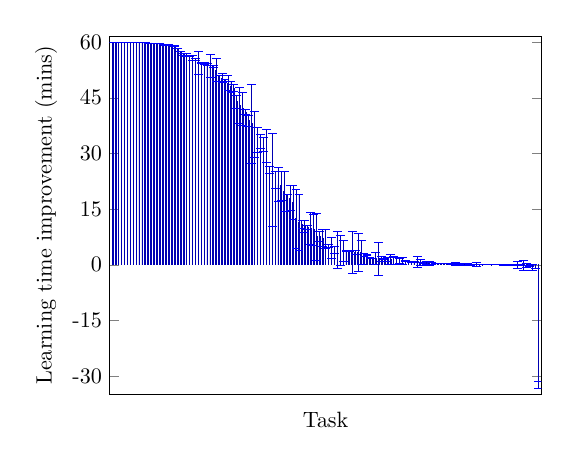
\begin{tikzpicture}[scale=0.8]
\begin{axis}[
ybar, 
bar width=.1mm, 
% width=10cm,
xmin=-1, 
xmax=145,
ymax=3700,
ymin=-2100,
ylabel={Learning time improvement (mins)},
ytick={-3600, -2700, -1800, -900, 0, 900, 1800, 2700, 3600},
yticklabels={-60, -45, -30, -15, 0, 15, 30, 45, 60},
xlabel={Task},
xtick=\empty,
xticklabel=\empty,
]
\addplot+[draw=blue!70!black, fill=blue!70!black,, error bars/.cd, y dir=both, y explicit] coordinates {
% \addplot+[draw=blue!70!black, fill=blue!70!black] coordinates {
(0, 3598) +- (0, 0)
(1, 3597) +- (0, 0)
(2, 3596) +- (0, 0)
(3, 3595) +- (0, 0)
(4, 3595) +- (0, 0)
(5, 3595) +- (0, 0)
(6, 3594) +- (0, 0)
(7, 3593) +- (0, 0)
(8, 3591) +- (0, 0)
(9, 3590) +- (0, 0)
(10, 3589) +- (0, 0)
(11, 3588) +- (0, 0)
(12, 3587) +- (0, 0)
(13, 3587) +- (0, 0)
(14, 3586) +- (0, 0)
(15, 3582) +- (0, 0)
(16, 3579) +- (0, 1)
(17, 3571) +- (0, 0)
(18, 3558) +- (0, 5)
(19, 3555) +- (0, 2)
(20, 3544) +- (0, 1)
(21, 3543) +- (0, 4)
(22, 3497) +- (0, 2)
(23, 3446) +- (0, 2)
(24, 3407) +- (0, 16)
(25, 3398) +- (0, 26)
(26, 3375) +- (0, 11)
(27, 3340) +- (0, 39)
(28, 3325) +- (0, 16)
(29, 3264) +- (0, 185)
(30, 3264) +- (0, 12)
(31, 3257) +- (0, 20)
(32, 3241) +- (0, 10)
(33, 3216) +- (0, 185)
(34, 3208) +- (0, 19)
(35, 3149) +- (0, 181)
(36, 3057) +- (0, 0)
(37, 3020) +- (0, 67)
(38, 2985) +- (0, 18)
(39, 2939) +- (0, 125)
(40, 2878) +- (0, 92)
(41, 2858) +- (0, 61)
(42, 2634) +- (0, 103)
(43, 2581) +- (0, 293)
(44, 2522) +- (0, 270)
(45, 2465) +- (0, 41)
(46, 2328) +- (0, 92)
(47, 2280) +- (0, 638)
(48, 2109) +- (0, 365)
(49, 2018) +- (0, 198)
(50, 2000) +- (0, 114)
(51, 1952) +- (0, 115)
(52, 1919) +- (0, 270)
(53, 1536) +- (0, 56)
(54, 1372) +- (0, 750)
(55, 1369) +- (0, 141)
(56, 1297) +- (0, 280)
(57, 1279) +- (0, 236)
(58, 1187) +- (0, 317)
(59, 1131) +- (0, 0)
(60, 1081) +- (0, 199)
(61, 1014) +- (0, 273)
(62, 744) +- (0, 474)
(63, 680) +- (0, 453)
(64, 650) +- (0, 70)
(65, 623) +- (0, 101)
(66, 603) +- (0, 33)
(67, 587) +- (0, 255)
(68, 566) +- (0, 246)
(69, 456) +- (0, 379)
(70, 454) +- (0, 79)
(71, 429) +- (0, 140)
(72, 419) +- (0, 159)
(73, 305) +- (0, 18)
(74, 268) +- (0, 171)
(75, 246) +- (0, 58)
(76, 235) +- (0, 301)
(77, 233) +- (0, 238)
(78, 227) +- (0, 170)
(79, 224) +- (0, 12)
(80, 221) +- (0, 9)
(81, 205) +- (0, 342)
(82, 204) +- (0, 30)
(83, 194) +- (0, 307)
(84, 193) +- (0, 193)
(85, 161) +- (0, 30)
(86, 154) +- (0, 10)
(87, 110) +- (0, 15)
(88, 104) +- (0, 6)
(89, 103) +- (0, 103)
(90, 96) +- (0, 263)
(91, 95) +- (0, 34)
(92, 95) +- (0, 3)
(93, 89) +- (0, 30)
(94, 85) +- (0, 85)
(95, 65) +- (0, 62)
(96, 63) +- (0, 63)
(97, 63) +- (0, 35)
(98, 61) +- (0, 61)
(99, 60) +- (0, 3)
(100, 51) +- (0, 0)
(101, 50) +- (0, 4)
(102, 48) +- (0, 13)
(103, 47) +- (0, 96)
(104, 37) +- (0, 43)
(105, 31) +- (0, 2)
(106, 28) +- (0, 21)
(107, 24) +- (0, 31)
(108, 24) +- (0, 18)
(109, 23) +- (0, 5)
(110, 22) +- (0, 4)
(111, 21) +- (0, 1)
(112, 19) +- (0, 0)
(113, 17) +- (0, 3)
(114, 16) +- (0, 0)
(115, 15) +- (0, 10)
(116, 11) +- (0, 21)
(117, 10) +- (0, 4)
(118, 9) +- (0, 8)
(119, 8) +- (0, 11)
(120, 6) +- (0, 12)
(121, 5) +- (0, 8)
(122, 5) +- (0, 1)
(123, 4) +- (0, 27)
(124, 4) +- (0, 4)
(125, 3) +- (0, 2)
(126, 3) +- (0, 0)
(127, 3) +- (0, 0)
(128, 2) +- (0, 1)
(129, 2) +- (0, 0)
(130, 2) +- (0, 0)
(131, 2) +- (0, 0)
(132, -2) +- (0, 1)
(133, -2) +- (0, 0)
(134, -3) +- (0, 2)
(135, -3) +- (0, 2)
(136, -3) +- (0, 0)
(137, -4) +- (0, 59)
(138, -5) +- (0, 3)
(139, -12) +- (0, 84)
(140, -15) +- (0, 33)
(141, -17) +- (0, 5)
(142, -43) +- (0, 47)
(143, -59) +- (0, 5)
(144, -1941) +- (0, 56)
% (0, 3598) +- (0, 0)
% (1, 3597) +- (0, 0)
% (2, 3596) +- (0, 0)
% (3, 3595) +- (0, 0)
% (4, 3595) +- (0, 0)
% (5, 3595) +- (0, 0)
% (6, 3594) +- (0, 0)
% (7, 3593) +- (0, 0)
% (8, 3591) +- (0, 0)
% (9, 3590) +- (0, 0)
% (10, 3589) +- (0, 0)
% (11, 3588) +- (0, 0)
% (12, 3587) +- (0, 1)
% (13, 3587) +- (0, 0)
% (14, 3586) +- (0, 1)
% (15, 3583) +- (0, 1)
% (16, 3578) +- (0, 2)
% (17, 3570) +- (0, 1)
% (18, 3555) +- (0, 5)
% (19, 3553) +- (0, 11)
% (20, 3547) +- (0, 8)
% (21, 3546) +- (0, 1)
% (22, 3501) +- (0, 1)
% (23, 3442) +- (0, 1)
% (24, 3429) +- (0, 11)
% (25, 3385) +- (0, 1)
% (26, 3365) +- (0, 43)
% (27, 3362) +- (0, 133)
% (28, 3321) +- (0, 79)
% (29, 3318) +- (0, 37)
% (30, 3286) +- (0, 0)
% (31, 3253) +- (0, 19)
% (32, 3248) +- (0, 46)
% (33, 3232) +- (0, 10)
% (34, 3118) +- (0, 389)
% (35, 3094) +- (0, 388)
% (36, 3057) +- (0, 0)
% (37, 3050) +- (0, 380)
% (38, 2991) +- (0, 31)
% (39, 2954) +- (0, 134)
% (40, 2843) +- (0, 271)
% (41, 2811) +- (0, 33)
% (42, 2766) +- (0, 72)
% (43, 2765) +- (0, 50)
% (44, 2758) +- (0, 133)
% (45, 2673) +- (0, 206)
% (46, 2505) +- (0, 60)
% (47, 2395) +- (0, 6)
% (48, 2325) +- (0, 615)
% (49, 2281) +- (0, 314)
% (50, 2174) +- (0, 1324)
% (51, 2104) +- (0, 210)
% (52, 1762) +- (0, 75)
% (53, 1715) +- (0, 588)
% (54, 1650) +- (0, 140)
% (55, 1524) +- (0, 345)
% (56, 1477) +- (0, 85)
% (57, 1192) +- (0, 235)
% (58, 1131) +- (0, 0)
% (59, 1044) +- (0, 463)
% (60, 1000) +- (0, 632)
% (61, 866) +- (0, 428)
% (62, 818) +- (0, 27)
% (63, 769) +- (0, 37)
% (64, 732) +- (0, 195)
% (65, 717) +- (0, 542)
% (66, 640) +- (0, 64)
% (67, 590) +- (0, 498)
% (68, 499) +- (0, 184)
% (69, 489) +- (0, 371)
% (70, 429) +- (0, 140)
% (71, 428) +- (0, 318)
% (72, 408) +- (0, 316)
% (73, 387) +- (0, 387)
% (74, 334) +- (0, 20)
% (75, 259) +- (0, 87)
% (76, 237) +- (0, 59)
% (77, 233) +- (0, 14)
% (78, 231) +- (0, 360)
% (79, 229) +- (0, 19)
% (80, 193) +- (0, 59)
% (81, 164) +- (0, 21)
% (82, 149) +- (0, 14)
% (83, 122) +- (0, 122)
% (84, 122) +- (0, 122)
% (85, 118) +- (0, 52)
% (86, 113) +- (0, 6)
% (87, 96) +- (0, 23)
% (88, 96) +- (0, 7)
% (89, 95) +- (0, 95)
% (90, 94) +- (0, 74)
% (91, 92) +- (0, 170)
% (92, 64) +- (0, 0)
% (93, 58) +- (0, 97)
% (94, 58) +- (0, 32)
% (95, 54) +- (0, 6)
% (96, 52) +- (0, 1)
% (97, 47) +- (0, 111)
% (98, 42) +- (0, 36)
% (99, 42) +- (0, 19)
% (100, 36) +- (0, 27)
% (101, 33) +- (0, 4)
% (102, 32) +- (0, 2)
% (103, 29) +- (0, 1)
% (104, 24) +- (0, 2)
% (105, 21) +- (0, 10)
% (106, 20) +- (0, 15)
% (107, 18) +- (0, 0)
% (108, 17) +- (0, 5)
% (109, 16) +- (0, 1)
% (110, 13) +- (0, 30)
% (111, 12) +- (0, 9)
% (112, 11) +- (0, 1)
% (113, 7) +- (0, 3)
% (114, 4) +- (0, 8)
% (115, 4) +- (0, 3)
% (116, 3) +- (0, 4)
% (117, 3) +- (0, 2)
% (118, 3) +- (0, 2)
% (119, 3) +- (0, 1)
% (120, 3) +- (0, 1)
% (121, 3) +- (0, 0)
% (122, 3) +- (0, 0)
% (123, 2) +- (0, 10)
% (124, 2) +- (0, 8)
% (125, 2) +- (0, 6)
% (126, 2) +- (0, 2)
% (127, 2) +- (0, 2)
% (128, 2) +- (0, 1)
% (129, 2) +- (0, 1)
% (130, 2) +- (0, 1)
% (131, 2) +- (0, 0)
% (132, 2) +- (0, 0)
% (133, 2) +- (0, 0)
% (134, -2) +- (0, 4)
% (135, -2) +- (0, 2)
% (136, -2) +- (0, 1)
% (137, -2) +- (0, 1)
% (138, -2) +- (0, 1)
% (139, -2) +- (0, 0)
% (140, -3) +- (0, 3)
% (141, -4) +- (0, 6)
% (142, -8) +- (0, 4)
% (143, -9) +- (0, 39)
% (144, -10) +- (0, 3)
% (145, -11) +- (0, 14)
% (146, -15) +- (0, 28)
% (147, -15) +- (0, 10)
% (148, -41) +- (0, 106)
% (149, -49) +- (0, 134)
% (150, -58) +- (0, 9)
% (151, -60) +- (0, 37)
% (152, -104) +- (0, 155)
% (153, -316) +- (0, 261)
% (154, -2024) +- (0, 46)
};
\end{axis}
\end{tikzpicture}
\caption{Learning time improvement of \name{} compared to \popper{}.
In other words, this plot shows the learning time improvement when ignoring pointless rules.
The tasks are ordered by the learning time improvement.
For legibility, we only show tasks where the learning times differ by more than 1 second.
}
\label{fig:q1_times}
\end{figure}




Figure \ref{fig:q1_accs} shows the improvement in predictive accuracy of \name{} vs \popper{}.
In other words, Figure \ref{fig:q1_accs} shows the predictive accuracy improvement when ignoring pointless rules.
The results show that \name{} can drastically improve predictive accuracies. 
% McNeymar's test confirms ($p<0.01$) that \name{} improves predictive accuracies on \ac{24/42} tasks.
% McNeymar's test confirms ($p<0.01$) that \name{} reduces predictive accuracies on \ac{24/42} tasks.
Although both systems are guaranteed to learn optimal hypotheses, they are not guaranteed to find them given the time limit.
The reason \name{} often improves accuracy is that it finds a good hypothesis quicker than \popper{}.

\begin{figure}[h!]
\centering
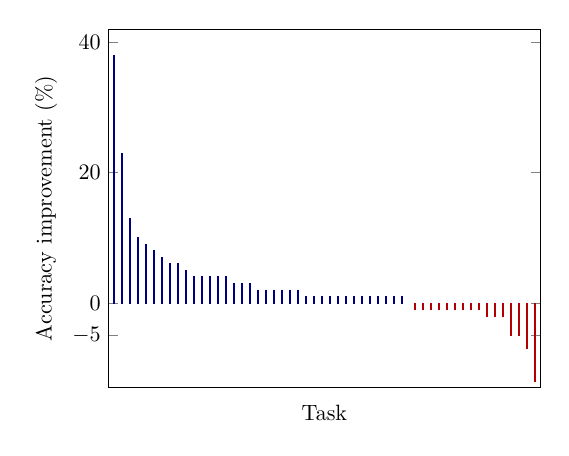
\begin{tikzpicture}[scale=0.8]
\begin{axis}[
ybar, 
% width=10cm,
% height=5cm,
bar width=.1mm, 
xmin=-1, 
xmax=53,
ymin=-13,
ymax=42,
ylabel={Accuracy improvement (\%)},
ytick={-5, 0, 20, 40},
% yticklabels={-60, -45, -30, -15, 0, 15, 30, 45, 60},
xlabel={Task},
xtick=\empty,
xticklabel=\empty,
]

% Positive values in blue

\addplot+[draw=blue!50!black, fill=blue!50!black] coordinates {
% \addplot+[] coordinates {
(0, 38) +- (0, 0)
(1, 23) +- (0, 0)
(2, 13) +- (0, 0)
(3, 10) +- (0, 0)
(4, 9) +- (0, 0)
(5, 8) +- (0, 0)
(6, 7) +- (0, 0)
(7, 6) +- (0, 0)
(8, 6) +- (0, 0)
(9, 5) +- (0, 0)
(10, 4) +- (0, 0)
(11, 4) +- (0, 0)
(12, 4) +- (0, 0)
(13, 4) +- (0, 0)
(14, 4) +- (0, 0)
(15, 3) +- (0, 0)
(16, 3) +- (0, 0)
(17, 3) +- (0, 0)
(18, 2) +- (0, 0)
(19, 2) +- (0, 0)
(20, 2) +- (0, 0)
(21, 2) +- (0, 0)
(22, 2) +- (0, 0)
(23, 2) +- (0, 0)
(24, 1) +- (0, 0)
(25, 1) +- (0, 0)
(26, 1) +- (0, 0)
(27, 1) +- (0, 0)
(28, 1) +- (0, 0)
(29, 1) +- (0, 0)
(30, 1) +- (0, 0)
(31, 1) +- (0, 0)
(32, 1) +- (0, 0)
(33, 1) +- (0, 0)
(34, 1) +- (0, 0)
(35, 1) +- (0, 0)
(36, 1) +- (0, 0)
};

% Negative values in red
\addplot+[draw=red!70!black, fill=red!70!black] coordinates {
(37, -1) +- (0, 0)
(38, -1) +- (0, 0)
(39, -1) +- (0, 0)
(40, -1) +- (0, 0)
(41, -1) +- (0, 0)
(42, -1) +- (0, 0)
(43, -1) +- (0, 0)
(44, -1) +- (0, 0)
(45, -1) +- (0, 0)
(46, -2) +- (0, 0)
(47, -2) +- (0, 0)
(48, -2) +- (0, 0)
(49, -5) +- (0, 0)
(50, -5) +- (0, 0)
(51, -7) +- (0, 0)
(52, -12) +- (0, 0)
};

\end{axis}



\end{tikzpicture}
\caption{Predictive accuracy improvement of \name{} compared to \popper{}, i.e. when ignoring pointless rules.}
\label{fig:q1_accs}
\end{figure}





\name{} can drastically improve learning performance.
For instance, consider the 1D-ARC task \emph{mirror}, shown in Figure \ref{fig:mirrorexs}.
% \ac{describe the task}
For this task, \name{} learns a hypothesis with 100\% predictive accuracy and terminates in 101 seconds.
By contrast, \popper{} learns a hypothesis with only 60\% accuracy and timeouts after 60 minutes.
In other words, on this task, ignoring pointless rules reduces learning times by at least 97\% and improves predictive accuracy by 40\%.
A reducible rule that \name{} finds on this task is:

\begin{center}
\begin{tabular}{l}
\emph{out(E,A,B) $\leftarrow$ succ(A,B), lt(C,A), lt(C,B)}\\
% \emph{h $\leftarrow$ add(A,V6,V1), add(V3,A,V1), add(V1,V3,A)}\\
% \emph{h $\leftarrow$ lt(V4,V1), in(V3,V2), lt(V3,V1), c0(V4)}\\
\end{tabular}
\end{center}

\noindent
This rule is reducible because if $B$ is the successor $A$ and $C$ is smaller than $A$ then $C$ must be smaller than $B$.
When \name{} identifies that this rule is pointless, it builds a constraint to prune all specialisations (supersets) from the hypothesis space. 
% \ac{discuss these pointless rules}

% \begin{center}
% \begin{tabular}{l}
% \ac{reducible 1}
% \end{tabular}
% \end{center}

% \begin{center}
% \begin{tabular}{l}
% \ac{reducible 1}
% \end{tabular}
% \end{center}


As a second example, in the IGGP dataset, one of the tasks is to learn a set of rules to describe a legal move in the \emph{eight puzzle} game.
For this task, both \name{} and \popper{} learn hypotheses with 100\% accuracy.
However, whereas \popper{} does not terminate (prove optimality) within 60 minutes, \name{} terminates (proves optimality) after only 10 seconds, a 99\% improvement.
A reducible rule that \name{} finds is:
\begin{center}
\begin{tabular}{l}
\emph{legal\_move(A,B,C,D) $\leftarrow$ succ(D,E), pos1(D), pos2(E)}
\end{tabular}
\end{center}

\noindent
This rule is reducible because the \emph{pos$_i$} relations denote positions in the game board, where 
\emph{pos$_i$} precedes \emph{pos$_{i+1}$}.
Therefore, if $pos_1(D)$ is true and $E$ is the successor of $D$ then $pos_2(E)$ must be true, and this literal is therefore redundant.

Three indiscriminate rules that \name{} finds are:
\begin{center}
\begin{tabular}{l}
\emph{legal\_move(A,B,C,D) $\leftarrow$ role(B)}\\
\emph{legal\_move(A,B,C,D) $\leftarrow$ index(C)}\\
\emph{legal\_move(A,B,C,D) $\leftarrow$ index(D)}\\
\end{tabular}
\end{center}

\noindent
These rules are indiscriminate because \emph{role(B)}, \emph{index(C)}, and \emph{index(D)} are true for every negative example and thus are redundant in the rule.

There is one noticeable exception (the rightmost bar) in Figure \ref{fig:q1_times} where \name{} is substantially worse than \popper{} (2160 seconds vs 86 seconds).
This task is \emph{pilgrimage-legal\_place\_pilgrim} from the IGGP dataset, where the mean overhead was 185s.
% \ac{need to check again over several runs}

Overall, the results in this section show that the answer to \textbf{Q1} is yes, identifying pointless can drastically improve learning times whilst maintaining high predictive accuracies. 


\subsubsection{Q2. What is the overhead of finding pointless rules?}

Figure \ref{fig:overhead} shows the ratio of learning time spent finding pointless rules.
The mean overhead is 2\%. 
The maximum is 80\%.
The overhead is less than 10\% on 85\% of the tasks.
Therefore, the results in this section show that the answer to \textbf{Q2} is that the overhead of identifying pointless is typically small ($<$10\%).

\begin{figure}[h!]
\centering
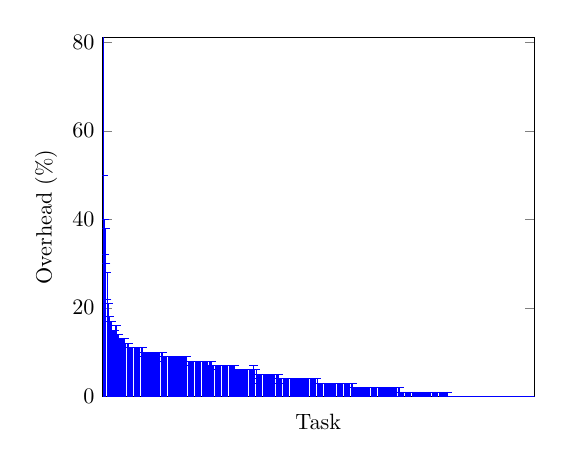
\begin{tikzpicture}[scale=0.8]
\begin{axis}[
ybar, 
bar width=.01mm, 
xmin=-1, 
xmax=367,
ymin=-0,
ymax=81,
ylabel={Overhead (\%)},
% ytick={0, 10, 20, 30, 40, 50},
% yticklabels={-60, -45, -30, -15, 0, 15, 30, 45, 60},
xlabel={Task},
xtick=\empty,
xticklabel=\empty,
]

\addplot+[error bars/.cd, y dir=both, y explicit] coordinates {
(0, 80) +- (0, 30)
(1, 36) +- (0, 4)
(2, 34) +- (0, 4)
(3, 25) +- (0, 3)
(4, 21) +- (0, 0)
(5, 18) +- (0, 0)
(6, 17) +- (0, 0)
(7, 16) +- (0, 1)
(8, 15) +- (0, 0)
(9, 15) +- (0, 0)
(10, 14) +- (0, 2)
(11, 14) +- (0, 2)
(12, 14) +- (0, 0)
(13, 13) +- (0, 1)
(14, 13) +- (0, 0)
(15, 13) +- (0, 0)
(16, 12) +- (0, 1)
(17, 12) +- (0, 1)
(18, 12) +- (0, 1)
(19, 12) +- (0, 0)
(20, 12) +- (0, 0)
(21, 12) +- (0, 0)
(22, 11) +- (0, 0)
(23, 11) +- (0, 0)
(24, 11) +- (0, 0)
(25, 11) +- (0, 0)
(26, 11) +- (0, 0)
(27, 11) +- (0, 0)
(28, 11) +- (0, 0)
(29, 11) +- (0, 0)
(30, 11) +- (0, 0)
(31, 10) +- (0, 1)
(32, 10) +- (0, 1)
(33, 10) +- (0, 1)
(34, 10) +- (0, 0)
(35, 10) +- (0, 0)
(36, 10) +- (0, 0)
(37, 10) +- (0, 0)
(38, 10) +- (0, 0)
(39, 10) +- (0, 0)
(40, 10) +- (0, 0)
(41, 10) +- (0, 0)
(42, 10) +- (0, 0)
(43, 10) +- (0, 0)
(44, 10) +- (0, 0)
(45, 10) +- (0, 0)
(46, 10) +- (0, 0)
(47, 9) +- (0, 1)
(48, 9) +- (0, 1)
(49, 9) +- (0, 1)
(50, 9) +- (0, 1)
(51, 9) +- (0, 0)
(52, 9) +- (0, 0)
(53, 9) +- (0, 0)
(54, 9) +- (0, 0)
(55, 9) +- (0, 0)
(56, 9) +- (0, 0)
(57, 9) +- (0, 0)
(58, 9) +- (0, 0)
(59, 9) +- (0, 0)
(60, 9) +- (0, 0)
(61, 9) +- (0, 0)
(62, 9) +- (0, 0)
(63, 9) +- (0, 0)
(64, 9) +- (0, 0)
(65, 9) +- (0, 0)
(66, 9) +- (0, 0)
(67, 9) +- (0, 0)
(68, 8) +- (0, 1)
(69, 8) +- (0, 1)
(70, 8) +- (0, 1)
(71, 8) +- (0, 1)
(72, 8) +- (0, 0)
(73, 8) +- (0, 0)
(74, 8) +- (0, 0)
(75, 8) +- (0, 0)
(76, 8) +- (0, 0)
(77, 8) +- (0, 0)
(78, 8) +- (0, 0)
(79, 8) +- (0, 0)
(80, 8) +- (0, 0)
(81, 8) +- (0, 0)
(82, 8) +- (0, 0)
(83, 8) +- (0, 0)
(84, 8) +- (0, 0)
(85, 8) +- (0, 0)
(86, 8) +- (0, 0)
(87, 8) +- (0, 0)
(88, 8) +- (0, 0)
(89, 7) +- (0, 1)
(90, 7) +- (0, 1)
(91, 7) +- (0, 1)
(92, 7) +- (0, 1)
(93, 7) +- (0, 0)
(94, 7) +- (0, 0)
(95, 7) +- (0, 0)
(96, 7) +- (0, 0)
(97, 7) +- (0, 0)
(98, 7) +- (0, 0)
(99, 7) +- (0, 0)
(100, 7) +- (0, 0)
(101, 7) +- (0, 0)
(102, 7) +- (0, 0)
(103, 7) +- (0, 0)
(104, 7) +- (0, 0)
(105, 7) +- (0, 0)
(106, 7) +- (0, 0)
(107, 7) +- (0, 0)
(108, 7) +- (0, 0)
(109, 7) +- (0, 0)
(110, 7) +- (0, 0)
(111, 7) +- (0, 0)
(112, 6) +- (0, 1)
(113, 6) +- (0, 0)
(114, 6) +- (0, 0)
(115, 6) +- (0, 0)
(116, 6) +- (0, 0)
(117, 6) +- (0, 0)
(118, 6) +- (0, 0)
(119, 6) +- (0, 0)
(120, 6) +- (0, 0)
(121, 6) +- (0, 0)
(122, 6) +- (0, 0)
(123, 6) +- (0, 0)
(124, 6) +- (0, 0)
(125, 6) +- (0, 0)
(126, 6) +- (0, 0)
(127, 6) +- (0, 0)
(128, 5) +- (0, 2)
(129, 5) +- (0, 1)
(130, 5) +- (0, 1)
(131, 5) +- (0, 0)
(132, 5) +- (0, 0)
(133, 5) +- (0, 0)
(134, 5) +- (0, 0)
(135, 5) +- (0, 0)
(136, 5) +- (0, 0)
(137, 5) +- (0, 0)
(138, 5) +- (0, 0)
(139, 5) +- (0, 0)
(140, 5) +- (0, 0)
(141, 5) +- (0, 0)
(142, 5) +- (0, 0)
(143, 5) +- (0, 0)
(144, 5) +- (0, 0)
(145, 5) +- (0, 0)
(146, 5) +- (0, 0)
(147, 5) +- (0, 0)
(148, 5) +- (0, 0)
(149, 4) +- (0, 1)
(150, 4) +- (0, 0)
(151, 4) +- (0, 0)
(152, 4) +- (0, 0)
(153, 4) +- (0, 0)
(154, 4) +- (0, 0)
(155, 4) +- (0, 0)
(156, 4) +- (0, 0)
(157, 4) +- (0, 0)
(158, 4) +- (0, 0)
(159, 4) +- (0, 0)
(160, 4) +- (0, 0)
(161, 4) +- (0, 0)
(162, 4) +- (0, 0)
(163, 4) +- (0, 0)
(164, 4) +- (0, 0)
(165, 4) +- (0, 0)
(166, 4) +- (0, 0)
(167, 4) +- (0, 0)
(168, 4) +- (0, 0)
(169, 4) +- (0, 0)
(170, 4) +- (0, 0)
(171, 4) +- (0, 0)
(172, 4) +- (0, 0)
(173, 4) +- (0, 0)
(174, 4) +- (0, 0)
(175, 4) +- (0, 0)
(176, 4) +- (0, 0)
(177, 4) +- (0, 0)
(178, 4) +- (0, 0)
(179, 4) +- (0, 0)
(180, 4) +- (0, 0)
(181, 4) +- (0, 0)
(182, 4) +- (0, 0)
(183, 3) +- (0, 0)
(184, 3) +- (0, 0)
(185, 3) +- (0, 0)
(186, 3) +- (0, 0)
(187, 3) +- (0, 0)
(188, 3) +- (0, 0)
(189, 3) +- (0, 0)
(190, 3) +- (0, 0)
(191, 3) +- (0, 0)
(192, 3) +- (0, 0)
(193, 3) +- (0, 0)
(194, 3) +- (0, 0)
(195, 3) +- (0, 0)
(196, 3) +- (0, 0)
(197, 3) +- (0, 0)
(198, 3) +- (0, 0)
(199, 3) +- (0, 0)
(200, 3) +- (0, 0)
(201, 3) +- (0, 0)
(202, 3) +- (0, 0)
(203, 3) +- (0, 0)
(204, 3) +- (0, 0)
(205, 3) +- (0, 0)
(206, 3) +- (0, 0)
(207, 3) +- (0, 0)
(208, 3) +- (0, 0)
(209, 3) +- (0, 0)
(210, 3) +- (0, 0)
(211, 3) +- (0, 0)
(212, 3) +- (0, 0)
(213, 2) +- (0, 0)
(214, 2) +- (0, 0)
(215, 2) +- (0, 0)
(216, 2) +- (0, 0)
(217, 2) +- (0, 0)
(218, 2) +- (0, 0)
(219, 2) +- (0, 0)
(220, 2) +- (0, 0)
(221, 2) +- (0, 0)
(222, 2) +- (0, 0)
(223, 2) +- (0, 0)
(224, 2) +- (0, 0)
(225, 2) +- (0, 0)
(226, 2) +- (0, 0)
(227, 2) +- (0, 0)
(228, 2) +- (0, 0)
(229, 2) +- (0, 0)
(230, 2) +- (0, 0)
(231, 2) +- (0, 0)
(232, 2) +- (0, 0)
(233, 2) +- (0, 0)
(234, 2) +- (0, 0)
(235, 2) +- (0, 0)
(236, 2) +- (0, 0)
(237, 2) +- (0, 0)
(238, 2) +- (0, 0)
(239, 2) +- (0, 0)
(240, 2) +- (0, 0)
(241, 2) +- (0, 0)
(242, 2) +- (0, 0)
(243, 2) +- (0, 0)
(244, 2) +- (0, 0)
(245, 2) +- (0, 0)
(246, 2) +- (0, 0)
(247, 2) +- (0, 0)
(248, 2) +- (0, 0)
(249, 2) +- (0, 0)
(250, 2) +- (0, 0)
(251, 1) +- (0, 1)
(252, 1) +- (0, 1)
(253, 1) +- (0, 0)
(254, 1) +- (0, 0)
(255, 1) +- (0, 0)
(256, 1) +- (0, 0)
(257, 1) +- (0, 0)
(258, 1) +- (0, 0)
(259, 1) +- (0, 0)
(260, 1) +- (0, 0)
(261, 1) +- (0, 0)
(262, 1) +- (0, 0)
(263, 1) +- (0, 0)
(264, 1) +- (0, 0)
(265, 1) +- (0, 0)
(266, 1) +- (0, 0)
(267, 1) +- (0, 0)
(268, 1) +- (0, 0)
(269, 1) +- (0, 0)
(270, 1) +- (0, 0)
(271, 1) +- (0, 0)
(272, 1) +- (0, 0)
(273, 1) +- (0, 0)
(274, 1) +- (0, 0)
(275, 1) +- (0, 0)
(276, 1) +- (0, 0)
(277, 1) +- (0, 0)
(278, 1) +- (0, 0)
(279, 1) +- (0, 0)
(280, 1) +- (0, 0)
(281, 1) +- (0, 0)
(282, 1) +- (0, 0)
(283, 1) +- (0, 0)
(284, 1) +- (0, 0)
(285, 1) +- (0, 0)
(286, 1) +- (0, 0)
(287, 1) +- (0, 0)
(288, 1) +- (0, 0)
(289, 1) +- (0, 0)
(290, 1) +- (0, 0)
(291, 1) +- (0, 0)
(292, 1) +- (0, 0)
(293, 1) +- (0, 0)
(294, 0) +- (0, 0)
(295, 0) +- (0, 0)
(296, 0) +- (0, 0)
(297, 0) +- (0, 0)
(298, 0) +- (0, 0)
(299, 0) +- (0, 0)
(300, 0) +- (0, 0)
(301, 0) +- (0, 0)
(302, 0) +- (0, 0)
(303, 0) +- (0, 0)
(304, 0) +- (0, 0)
(305, 0) +- (0, 0)
(306, 0) +- (0, 0)
(307, 0) +- (0, 0)
(308, 0) +- (0, 0)
(309, 0) +- (0, 0)
(310, 0) +- (0, 0)
(311, 0) +- (0, 0)
(312, 0) +- (0, 0)
(313, 0) +- (0, 0)
(314, 0) +- (0, 0)
(315, 0) +- (0, 0)
(316, 0) +- (0, 0)
(317, 0) +- (0, 0)
(318, 0) +- (0, 0)
(319, 0) +- (0, 0)
(320, 0) +- (0, 0)
(321, 0) +- (0, 0)
(322, 0) +- (0, 0)
(323, 0) +- (0, 0)
(324, 0) +- (0, 0)
(325, 0) +- (0, 0)
(326, 0) +- (0, 0)
(327, 0) +- (0, 0)
(328, 0) +- (0, 0)
(329, 0) +- (0, 0)
(330, 0) +- (0, 0)
(331, 0) +- (0, 0)
(332, 0) +- (0, 0)
(333, 0) +- (0, 0)
(334, 0) +- (0, 0)
(335, 0) +- (0, 0)
(336, 0) +- (0, 0)
(337, 0) +- (0, 0)
(338, 0) +- (0, 0)
(339, 0) +- (0, 0)
(340, 0) +- (0, 0)
(341, 0) +- (0, 0)
(342, 0) +- (0, 0)
(343, 0) +- (0, 0)
(344, 0) +- (0, 0)
(345, 0) +- (0, 0)
(346, 0) +- (0, 0)
(347, 0) +- (0, 0)
(348, 0) +- (0, 0)
(349, 0) +- (0, 0)
(350, 0) +- (0, 0)
(351, 0) +- (0, 0)
(352, 0) +- (0, 0)
(353, 0) +- (0, 0)
(354, 0) +- (0, 0)
(355, 0) +- (0, 0)
(356, 0) +- (0, 0)
(357, 0) +- (0, 0)
(358, 0) +- (0, 0)
(359, 0) +- (0, 0)
(360, 0) +- (0, 0)
(361, 0) +- (0, 0)
(362, 0) +- (0, 0)
(363, 0) +- (0, 0)
(364, 0) +- (0, 0)
(365, 0) +- (0, 0)
(366, 0) +- (0, 0)
% (0, 49) +- (0, 3)
% (1, 38) +- (0, 9)
% (2, 30) +- (0, 4)
% (3, 26) +- (0, 2)
% (4, 20) +- (0, 0)
% (5, 18) +- (0, 1)
% (6, 18) +- (0, 0)
% (7, 17) +- (0, 0)
% (8, 16) +- (0, 0)
% (9, 15) +- (0, 3)
% (10, 15) +- (0, 2)
% (11, 15) +- (0, 0)
% (12, 14) +- (0, 0)
% (13, 14) +- (0, 0)
% (14, 14) +- (0, 0)
% (15, 12) +- (0, 2)
% (16, 12) +- (0, 2)
% (17, 12) +- (0, 1)
% (18, 12) +- (0, 0)
% (19, 12) +- (0, 0)
% (20, 12) +- (0, 0)
% (21, 12) +- (0, 0)
% (22, 12) +- (0, 0)
% (23, 11) +- (0, 2)
% (24, 11) +- (0, 1)
% (25, 11) +- (0, 1)
% (26, 11) +- (0, 0)
% (27, 11) +- (0, 0)
% (28, 11) +- (0, 0)
% (29, 11) +- (0, 0)
% (30, 11) +- (0, 0)
% (31, 10) +- (0, 2)
% (32, 10) +- (0, 1)
% (33, 10) +- (0, 1)
% (34, 10) +- (0, 1)
% (35, 10) +- (0, 1)
% (36, 10) +- (0, 0)
% (37, 10) +- (0, 0)
% (38, 10) +- (0, 0)
% (39, 10) +- (0, 0)
% (40, 10) +- (0, 0)
% (41, 10) +- (0, 0)
% (42, 10) +- (0, 0)
% (43, 10) +- (0, 0)
% (44, 10) +- (0, 0)
% (45, 10) +- (0, 0)
% (46, 10) +- (0, 0)
% (47, 10) +- (0, 0)
% (48, 10) +- (0, 0)
% (49, 10) +- (0, 0)
% (50, 10) +- (0, 0)
% (51, 10) +- (0, 0)
% (52, 10) +- (0, 0)
% (53, 9) +- (0, 1)
% (54, 9) +- (0, 1)
% (55, 9) +- (0, 0)
% (56, 9) +- (0, 0)
% (57, 9) +- (0, 0)
% (58, 9) +- (0, 0)
% (59, 9) +- (0, 0)
% (60, 9) +- (0, 0)
% (61, 9) +- (0, 0)
% (62, 9) +- (0, 0)
% (63, 9) +- (0, 0)
% (64, 9) +- (0, 0)
% (65, 9) +- (0, 0)
% (66, 9) +- (0, 0)
% (67, 9) +- (0, 0)
% (68, 9) +- (0, 0)
% (69, 8) +- (0, 2)
% (70, 8) +- (0, 1)
% (71, 8) +- (0, 1)
% (72, 8) +- (0, 1)
% (73, 8) +- (0, 1)
% (74, 8) +- (0, 1)
% (75, 8) +- (0, 1)
% (76, 8) +- (0, 0)
% (77, 8) +- (0, 0)
% (78, 8) +- (0, 0)
% (79, 8) +- (0, 0)
% (80, 8) +- (0, 0)
% (81, 8) +- (0, 0)
% (82, 8) +- (0, 0)
% (83, 8) +- (0, 0)
% (84, 8) +- (0, 0)
% (85, 8) +- (0, 0)
% (86, 8) +- (0, 0)
% (87, 8) +- (0, 0)
% (88, 8) +- (0, 0)
% (89, 8) +- (0, 0)
% (90, 8) +- (0, 0)
% (91, 7) +- (0, 2)
% (92, 7) +- (0, 2)
% (93, 7) +- (0, 1)
% (94, 7) +- (0, 1)
% (95, 7) +- (0, 1)
% (96, 7) +- (0, 0)
% (97, 7) +- (0, 0)
% (98, 7) +- (0, 0)
% (99, 7) +- (0, 0)
% (100, 7) +- (0, 0)
% (101, 7) +- (0, 0)
% (102, 7) +- (0, 0)
% (103, 7) +- (0, 0)
% (104, 7) +- (0, 0)
% (105, 7) +- (0, 0)
% (106, 7) +- (0, 0)
% (107, 7) +- (0, 0)
% (108, 7) +- (0, 0)
% (109, 6) +- (0, 5)
% (110, 6) +- (0, 2)
% (111, 6) +- (0, 1)
% (112, 6) +- (0, 1)
% (113, 6) +- (0, 1)
% (114, 6) +- (0, 1)
% (115, 6) +- (0, 1)
% (116, 6) +- (0, 1)
% (117, 6) +- (0, 0)
% (118, 6) +- (0, 0)
% (119, 6) +- (0, 0)
% (120, 6) +- (0, 0)
% (121, 6) +- (0, 0)
% (122, 6) +- (0, 0)
% (123, 6) +- (0, 0)
% (124, 6) +- (0, 0)
% (125, 6) +- (0, 0)
% (126, 6) +- (0, 0)
% (127, 6) +- (0, 0)
% (128, 6) +- (0, 0)
% (129, 6) +- (0, 0)
% (130, 6) +- (0, 0)
% (131, 6) +- (0, 0)
% (132, 6) +- (0, 0)
% (133, 6) +- (0, 0)
% (134, 5) +- (0, 1)
% (135, 5) +- (0, 1)
% (136, 5) +- (0, 0)
% (137, 5) +- (0, 0)
% (138, 5) +- (0, 0)
% (139, 5) +- (0, 0)
% (140, 5) +- (0, 0)
% (141, 5) +- (0, 0)
% (142, 5) +- (0, 0)
% (143, 5) +- (0, 0)
% (144, 5) +- (0, 0)
% (145, 5) +- (0, 0)
% (146, 5) +- (0, 0)
% (147, 5) +- (0, 0)
% (148, 5) +- (0, 0)
% (149, 5) +- (0, 0)
% (150, 5) +- (0, 0)
% (151, 5) +- (0, 0)
% (152, 4) +- (0, 2)
% (153, 4) +- (0, 1)
% (154, 4) +- (0, 1)
% (155, 4) +- (0, 0)
% (156, 4) +- (0, 0)
% (157, 4) +- (0, 0)
% (158, 4) +- (0, 0)
% (159, 4) +- (0, 0)
% (160, 4) +- (0, 0)
% (161, 4) +- (0, 0)
% (162, 4) +- (0, 0)
% (163, 4) +- (0, 0)
% (164, 4) +- (0, 0)
% (165, 4) +- (0, 0)
% (166, 4) +- (0, 0)
% (167, 4) +- (0, 0)
% (168, 4) +- (0, 0)
% (169, 4) +- (0, 0)
% (170, 4) +- (0, 0)
% (171, 4) +- (0, 0)
% (172, 4) +- (0, 0)
% (173, 4) +- (0, 0)
% (174, 4) +- (0, 0)
% (175, 4) +- (0, 0)
% (176, 4) +- (0, 0)
% (177, 4) +- (0, 0)
% (178, 4) +- (0, 0)
% (179, 4) +- (0, 0)
% (180, 4) +- (0, 0)
% (181, 4) +- (0, 0)
% (182, 4) +- (0, 0)
% (183, 4) +- (0, 0)
% (184, 4) +- (0, 0)
% (185, 4) +- (0, 0)
% (186, 4) +- (0, 0)
% (187, 3) +- (0, 2)
% (188, 3) +- (0, 0)
% (189, 3) +- (0, 0)
% (190, 3) +- (0, 0)
% (191, 3) +- (0, 0)
% (192, 3) +- (0, 0)
% (193, 3) +- (0, 0)
% (194, 3) +- (0, 0)
% (195, 3) +- (0, 0)
% (196, 3) +- (0, 0)
% (197, 3) +- (0, 0)
% (198, 3) +- (0, 0)
% (199, 3) +- (0, 0)
% (200, 3) +- (0, 0)
% (201, 3) +- (0, 0)
% (202, 3) +- (0, 0)
% (203, 3) +- (0, 0)
% (204, 3) +- (0, 0)
% (205, 3) +- (0, 0)
% (206, 3) +- (0, 0)
% (207, 3) +- (0, 0)
% (208, 3) +- (0, 0)
% (209, 3) +- (0, 0)
% (210, 3) +- (0, 0)
% (211, 3) +- (0, 0)
% (212, 3) +- (0, 0)
% (213, 3) +- (0, 0)
% (214, 3) +- (0, 0)
% (215, 3) +- (0, 0)
% (216, 2) +- (0, 2)
% (217, 2) +- (0, 1)
% (218, 2) +- (0, 1)
% (219, 2) +- (0, 1)
% (220, 2) +- (0, 0)
% (221, 2) +- (0, 0)
% (222, 2) +- (0, 0)
% (223, 2) +- (0, 0)
% (224, 2) +- (0, 0)
% (225, 2) +- (0, 0)
% (226, 2) +- (0, 0)
% (227, 2) +- (0, 0)
% (228, 2) +- (0, 0)
% (229, 2) +- (0, 0)
% (230, 2) +- (0, 0)
% (231, 2) +- (0, 0)
% (232, 2) +- (0, 0)
% (233, 2) +- (0, 0)
% (234, 2) +- (0, 0)
% (235, 2) +- (0, 0)
% (236, 2) +- (0, 0)
% (237, 2) +- (0, 0)
% (238, 2) +- (0, 0)
% (239, 2) +- (0, 0)
% (240, 2) +- (0, 0)
% (241, 2) +- (0, 0)
% (242, 2) +- (0, 0)
% (243, 2) +- (0, 0)
% (244, 2) +- (0, 0)
% (245, 2) +- (0, 0)
% (246, 2) +- (0, 0)
% (247, 2) +- (0, 0)
% (248, 2) +- (0, 0)
% (249, 2) +- (0, 0)
% (250, 2) +- (0, 0)
% (251, 1) +- (0, 1)
% (252, 1) +- (0, 0)
% (253, 1) +- (0, 0)
% (254, 1) +- (0, 0)
% (255, 1) +- (0, 0)
% (256, 1) +- (0, 0)
% (257, 1) +- (0, 0)
% (258, 1) +- (0, 0)
% (259, 1) +- (0, 0)
% (260, 1) +- (0, 0)
% (261, 1) +- (0, 0)
% (262, 1) +- (0, 0)
% (263, 1) +- (0, 0)
% (264, 1) +- (0, 0)
% (265, 1) +- (0, 0)
% (266, 1) +- (0, 0)
% (267, 1) +- (0, 0)
% (268, 1) +- (0, 0)
% (269, 1) +- (0, 0)
% (270, 1) +- (0, 0)
% (271, 1) +- (0, 0)
% (272, 1) +- (0, 0)
% (273, 1) +- (0, 0)
% (274, 1) +- (0, 0)
% (275, 1) +- (0, 0)
% (276, 1) +- (0, 0)
% (277, 1) +- (0, 0)
% (278, 1) +- (0, 0)
% (279, 1) +- (0, 0)
% (280, 1) +- (0, 0)
% (281, 1) +- (0, 0)
% (282, 1) +- (0, 0)
% (283, 1) +- (0, 0)
% (284, 1) +- (0, 0)
% (285, 1) +- (0, 0)
% (286, 1) +- (0, 0)
% (287, 1) +- (0, 0)
% (288, 1) +- (0, 0)
% (289, 1) +- (0, 0)
% (290, 1) +- (0, 0)
% (291, 0) +- (0, 0)
% (292, 0) +- (0, 0)
% (293, 0) +- (0, 0)
% (294, 0) +- (0, 0)
% (295, 0) +- (0, 0)
% (296, 0) +- (0, 0)
% (297, 0) +- (0, 0)
% (298, 0) +- (0, 0)
% (299, 0) +- (0, 0)
% (300, 0) +- (0, 0)
% (301, 0) +- (0, 0)
% (302, 0) +- (0, 0)
% (303, 0) +- (0, 0)
% (304, 0) +- (0, 0)
% (305, 0) +- (0, 0)
% (306, 0) +- (0, 0)
% (307, 0) +- (0, 0)
% (308, 0) +- (0, 0)
% (309, 0) +- (0, 0)
% (310, 0) +- (0, 0)
% (311, 0) +- (0, 0)
% (312, 0) +- (0, 0)
% (313, 0) +- (0, 0)
% (314, 0) +- (0, 0)
% (315, 0) +- (0, 0)
% (316, 0) +- (0, 0)
% (317, 0) +- (0, 0)
% (318, 0) +- (0, 0)
% (319, 0) +- (0, 0)
% (320, 0) +- (0, 0)
% (321, 0) +- (0, 0)
% (322, 0) +- (0, 0)
% (323, 0) +- (0, 0)
% (324, 0) +- (0, 0)
% (325, 0) +- (0, 0)
% (326, 0) +- (0, 0)
% (327, 0) +- (0, 0)
% (328, 0) +- (0, 0)
% (329, 0) +- (0, 0)
% (330, 0) +- (0, 0)
% (331, 0) +- (0, 0)
% (332, 0) +- (0, 0)
% (333, 0) +- (0, 0)
% (334, 0) +- (0, 0)
% (335, 0) +- (0, 0)
% (336, 0) +- (0, 0)
% (337, 0) +- (0, 0)
% (338, 0) +- (0, 0)
% (339, 0) +- (0, 0)
% (340, 0) +- (0, 0)
% (341, 0) +- (0, 0)
% (342, 0) +- (0, 0)
% (343, 0) +- (0, 0)
% (344, 0) +- (0, 0)
% (345, 0) +- (0, 0)
% (346, 0) +- (0, 0)
% (347, 0) +- (0, 0)
% (348, 0) +- (0, 0)

};
\end{axis}
\end{tikzpicture}
\caption{Overhead of finding pointless rules.}
\label{fig:overhead}
\end{figure}


\subsubsection{Q3. How Does \name{} compare to other approaches?}

Table \ref{tab:agg_acc} shows the predictive accuracies aggregated per domain of all the systems.
\name{} has higher predictive accuracy than \ale{} and \aspsynth{} on every domain.
\name{} has higher or equal predictive accuracy than \popper{} on every domain, within the margin of error.
These results suggest that the answer to \textbf{Q3} is that \name{} compares favourably to existing approaches in terms of predictive accuracies.

\begin{table}[ht]
\small
\centering
\begin{tabular}{@{}l|cccc@{}}
\textbf{Task} & \textbf{\ale{}} & \textbf{\aspsynth{}} & \textbf{\popper{}} & \textbf{\name{}}\\
\midrule
% \emph{imdb} & 50 & 50 & 100 & 100\\
% \emph{alzheimer} & 50 & 50 & 71 & 71\\
% \emph{jr} & 57 & 50 & 96 & 96\\
% \emph{trains} & 50 & 71 & 93 & 89\\
% \emph{1d} & 52 & 50 & 91 & 89\\
% \emph{zendo} & 50 & 72 & 92 & 96\\
% \emph{iggp} & 65 & 59 & 86 & 86\\
\emph{1d} & 52 $\pm$ 2 & 89 $\pm$ 2 & 93 $\pm$ 0 & 92 $\pm$ 0\\
\emph{alzheimer} & 52 $\pm$ 0 & 57 $\pm$ 1 & 74 $\pm$ 1 & 75 $\pm$ 1\\
\emph{iggp} & 58 $\pm$ 5 & 68 $\pm$ 0 & 85 $\pm$ 0 & 85 $\pm$ 0\\
\emph{imdb} & 61 $\pm$ 5 & 98 $\pm$ 0 & 100 $\pm$ 0 & 100 $\pm$ 0\\
\emph{jr} & 55 $\pm$ 5 & 83 $\pm$ 1 & 97 $\pm$ 0 & 97 $\pm$ 0\\
\emph{trains} & 50 $\pm$ 0 & 76 $\pm$ 1 & 87 $\pm$ 5 & 94 $\pm$ 3\\
\emph{zendo} & 53 $\pm$ 3 & 82 $\pm$ 0 & 84 $\pm$ 1 & 84 $\pm$ 1\\
\end{tabular}
\caption{
Aggregated predictive accuracies (\%) with a 600s timeout.
}
\label{tab:agg_acc}
\end{table}
% \dc{purely to show things are not damage by reducer. Point of predicative accuracy.}

% The results in Table \ref{tab:qaccs} show that \name{} has equal or higher predictive accuracy than \disco{} on all the domains. 
% Table \ref{tab:sota_times} shows the learning times aggregated per domain for \name{} and \disco{}.
% The results show that \name{} outperforms \disco{} in 6/8 domains and that they are matched in the other two domains.
% A paired t-test confirms the significance of the difference ($p < 0.01$). 
% \name{} can reduce learning times by 97\% compared to \disco{}, such as on the \emph{sql} domain.
% Overall, these results suggest that the answer to \textbf{Q3} is that \name{} compares favourably to existing approaches, both in terms of predictive accuracies and learning times.
\section{Conclusions and Limitations}

We have introduced an approach that identifies and ignores pointless (reducible and indiscriminate) rules.
We have shown that ignoring pointless rules is optimally sound (Propositions \ref{prop:sound_sat3} and \ref{prop:sound_Indiscriminate}).
We implemented our approach in \name{}, which identifies pointless rules in hypotheses and builds constraints from them to prune the hypothesis space.
We have proven that \name{} always learns an optimal hypothesis if one exists (Theorem \ref{thm:optcorrect}).
We have experimentally shown on multiple domains, including visual reasoning and game playing, that our approach can reduce learning times by 99\% whilst maintaining high predictive accuracies.

\subsection*{Limitations}

\textbf{Other systems.} 
The benefits of ignoring pointless rules should generalise to other ILP approaches.
For instance, the improvements should directly improve other LFF approaches, such as \textsc{hopper} \cite{hopper}, which learns higher-order programs, and \textsc{propper} \cite{propper}, which uses neurosymbolic inference to learn programs from probabilistic data.
Future would should empirically show the benefits in these systems.

% \textbf{Completeness/More pointless programs.} 
\section*{Acknowledgments}
Andrew Cropper was supported by the EPSRC fellowship (\emph{EP/V040340/1}). 
David M. Cerna was supported by the Czech Science Foundation Grant 22-06414L and Cost Action CA20111 EuroProofNet.


%% The file named.bst is a bibliography style file for BibTeX 0.99c
\bibliographystyle{named}
\bibliography{ijcai24}
\newpage
\hspace{.5em}
\newpage
\appendix
\section{Terminology}
\label{sec:terminology}
\subsection{Logic Programming}
We assume familiarity with logic programming \cite{lloyd:book} but restate some key relevant notation. A \emph{variable} is a string of characters starting with an uppercase letter. A \emph{predicate} symbol is a string of characters starting with a lowercase letter. The \emph{arity} $n$ of a function or predicate symbol is the number of arguments it takes. An \emph{atom} is a tuple $p(t_1, ..., t_n)$, where $p$ is a predicate of arity $n$ and $t_1$, ..., $t_n$ are terms, either variables or constants. An atom is \emph{ground} if it contains no variables. A \emph{literal} is an atom or the negation of an atom. A \emph{clause} is a set of literals.
A \emph{clausal theory} is a set of clauses. A \emph{constraint} is a clause without a non-negated literal. A \emph{definite} rule is a clause with exactly one non-negated literal. A \emph{program} is a set of definite rules. A \emph{substitution} $\theta = \{v_1 / t_1, ..., v_n/t_n \}$ is the simultaneous replacement of each variable $v_i$ by its corresponding term $t_i$.
A rule $c_1$ \emph{subsumes} a rule $c_2$ if and only if there exists a substitution $\theta$ such that $c_1 \theta \subseteq c_2$.
A program $h_1$ subsumes a program $h_2$, denoted $h_1 \preceq h_2$, if and only if $\forall c_2 \in h_2, \exists c_1 \in h_1$ such that $c_1$ subsumes $c_2$. A program $h_1$ is a \emph{specialisation} of a program $h_2$ if and only if $h_2 \preceq h_1$. A program $h_1$ is a \emph{generalisation} of a program $h_2$ if and only if $h_1 \preceq h_2$.
\subsection{Answer Set Programming}
We also assume familiarity with answer set programming \cite{asp} but restate some key relevant notation \cite{ilasp}.
A \emph{literal} can be either an atom $p$ or its \emph{default negation} $\text{not } p$ (often called \emph{negation by failure}). A normal rule is of the form $h \leftarrow b_1, ..., b_n, \text{not } c_1,... \text{not } c_m$. where $h$ is the \emph{head} of the rule, $b_1, ..., b_n, \text{not } c_1,... \text{not } c_m$ (collectively) is the \emph{body} of the rule, and all $h$, $b_i$, and $c_j$ are atoms. A \emph{constraint} is of the form $\leftarrow b_1, ..., b_n, \text{not } c_1,... \text{not } c_m.$ where the empty head means false. A \emph{choice rule} is an expression of the form $l\{h_1,...,h_m\}u \leftarrow b_1,...,b_n, \text{not } c_1,... \text{not } c_m$ where the head $l\{h_1,...,h_m\}u$ is called an \emph{aggregate}. In an aggregate, $l$ and $u$ are integers and $h_i$, for $1 \leq i \leq m$, are atoms. An \emph{answer set program} $P$ is a finite set of normal rules, constraints, and choice rules. Given an answer set program $P$, the \emph{Herbrand base} of $P$, denoted
as ${HB}_P$, is the set of all ground (variable free) atoms that can be formed from the predicates and constants that appear in $P$. When $P$ includes only normal rules, a set $A \in {HB}_P$ is an \emph{answer set} of $P$ iff it is the minimal model of the  \emph{reduct} $P^A$, which is the program constructed from the grounding of $P$ by first removing any rule whose body contains a literal $\text{not } c_i$ where $c_i \in A$, and then removing any defaultly negated literals in the remaining rules. An answer set $A$ satisfies a ground constraint $\leftarrow b_1, ..., b_n, \text{not } c_1,... \text{not } c_m.$ if it is not the case that $\{b_1, ..., b_n\} \in A$ and $A \cap \{c_1, ..., c_m\} = \emptyset$.


\end{document}


